%----------------------------------------------------------------------------------------
%	PACKAGES AND OTHER DOCUMENT CONFIGURATIONS
%----------------------------------------------------------------------------------------

\documentclass{tufte-book} % Use the tufte-book class
\usepackage{microtype} % Improves character and word spacing
\usepackage{multirow}

\usepackage{setspace} 
\usepackage{subfig}

\usepackage{tabularx}

\usepackage{fontawesome5}

\setcounter{secnumdepth}{1}

\usepackage{hyperref}
\hypersetup{colorlinks} % For colored links

\usepackage{ragged2e}
\usepackage{float}
\usepackage{amsmath}

\usepackage{enumerate}

\usepackage{caption}

\PassOptionsToPackage{usenames,dvipsnames,svgnames,table}{xcolor}
\usepackage[table]{xcolor}

\usepackage{colortbl}
\definecolor{lightgray}{gray}{0.9}

\usepackage[export]{adjustbox}
\usepackage{booktabs} % Better horizontal rules in tables

\usepackage{graphicx} % Needed to insert images into the document
\setkeys{Gin}{width=\linewidth,totalheight=\textheight,keepaspectratio} % Improves figure scaling

\usepackage{fancyvrb} % Allows customization of verbatim environments
\fvset{fontsize=\normalsize} % The font size of all verbatim text can be changed here

\usepackage{acro}
\DeclareAcronym{DTMF}{
  short=DTMF,
  long=Dual Tone Multi Frequncy,
}
\DeclareAcronym{PWM}{
  short=PWM,
  long=Pulse With Modulation,
}
\DeclareAcronym{IC}{
  short=IC,
  long=Integrated Circuits,
}
\DeclareAcronym{IR}{
  short=IR,
  long=Infra-Red,
}
\DeclareAcronym{LDR}{
  short=LDR,
  long=Light Dependent Resistor,
}
\DeclareAcronym{EMR}{
  short=EMR,
  long=Electro Magnetic Radiation,
}
\DeclareAcronym{PIR}{
  short=PIR,
  long=Passive Infrared,
}
\DeclareAcronym{IDE}{
  short=IDE,
  long=Integrated Development Environment,
}
\DeclareAcronym{IoT}{
  short=IoT,
  long=Internet of Things,
}
\DeclareAcronym{SBC}{
    short=SBC,
    long=Single Board Computer,
}
\DeclareAcronym{SoC}{
    short=SoC,
    long=System on Chip,
}
\DeclareAcronym{ADC}{
    short=ADC,
    long=Analog to Digital Conversion,
}

\usepackage{listings}   %configuration for codes
\definecolor{mGreen}{rgb}{0,0.6,0}
\definecolor{mGray}{rgb}{0.5,0.5,0.5}
\definecolor{mPurple}{rgb}{0.58,0,0.82}
\definecolor{backgroundColour}{rgb}{0.95,0.95,0.92}
\lstdefinestyle{CStyle}{
    backgroundcolor=\color{backgroundColour},   
    commentstyle=\color{mGreen},
    keywordstyle=\color{magenta},
    numberstyle=\tiny\color{mGray},
    stringstyle=\color{mPurple},
    basicstyle=\footnotesize,
    breakatwhitespace=false,         
    breaklines=true,                 
    captionpos=b,                    
    keepspaces=true,                 
    numbers=left,                    
    numbersep=5pt,                  
    showspaces=false,                
    showstringspaces=false,
    showtabs=false,                  
    tabsize=2,
    language=C
}

\def\ci#1{\textcircled{\resizebox{.5em}{!}{#1}}} 

\newcommand\Tstrut{\rule{0pt}{2.6ex}}       % "top" strut
\newcommand\Bstrut{\rule[-0.9ex]{0pt}{0pt}} % "bottom" strut
\newcommand{\TBstrut}{\Tstrut\Bstrut} % top&bottom struts

\newcommand{\hangp}[1]{\makebox[0pt][r]{(}#1\makebox[0pt][l]{)}} % New command to create parentheses around text in tables which take up no horizontal space - this improves column spacing
\newcommand{\hangstar}{\makebox[0pt][l]{*}} % New command to create asterisks in tables which take up no horizontal space - this improves column spacing

\usepackage{xspace} % Used for printing a trailing space better than using a tilde (~) using the \xspace command

\newcommand{\monthyear}{\ifcase\month\or January\or February\or March\or April\or May\or June\or July\or August\or September\or October\or November\or December\fi\space\number\year} % A command to print the current month and year

\newcommand{\blankpage}{\newpage\hbox{}\thispagestyle{empty}\newpage} % Command to insert a blank page

\usepackage{makeidx} % Used to generate the index
\makeindex % Generate the index which is printed at the end of the document



%----------------------------------------------------------------------------------------
%	BOOK META-INFORMATION
%----------------------------------------------------------------------------------------

\title{ACTUATOR : Stepping into ROBOTICS} % Title of the book

\author{ROBOCEK Project Developers} % Author

\publisher{ROBOCEK 2020-21} % Publisher

%----------------------------------------------------------------------------------------
\begin{document}
\frontmatter

%----------------------------------------------------------------------------------------
%	COVER PAGE
%----------------------------------------------------------------------------------------

%----------------------------------------------------------------------------------------
%	TITLE
%----------------------------------------------------------------------------------------
\maketitle

%----------------------------------------------------------------------------------------
%	COPYRIGHT PAGE
%----------------------------------------------------------------------------------------
\newpage
\begin{fullwidth}
~\vfill
\thispagestyle{empty}
\setlength{\parindent}{0pt}
\setlength{\parskip}{\baselineskip}
Copyright \copyright\ \the\year\ \thanklessauthor

\par\smallcaps{Published by \thanklesspublisher}

\par\smallcaps{robocek.org}

\par Licensed under the Apache License, Version 2.0 (the ``License''); you may not use this file except in compliance with the License. You may obtain a copy of the License at \url{http://www.apache.org/licenses/LICENSE-2.0}. Unless required by applicable law or agreed to in writing, software distributed under the License is distributed on an \smallcaps{``AS IS'' BASIS, WITHOUT WARRANTIES OR CONDITIONS OF ANY KIND}, either express or implied. See the License for the specific language governing permissions and limitations under the License.\index{license}

\par\textit{First printing, \monthyear}
\end{fullwidth}

%----------------------------------------------------------------------------------------
%	IMPRINT : About the publisher
%----------------------------------------------------------------------------------------

%----------------------------------------------------------------------------------------
%	Epigraph : A quotation
%----------------------------------------------------------------------------------------
\newpage
~\vfill
\begin{fullwidth}
    \noindent\fontsize{18}{22}\selectfont\itshape \nohyphenation
    There are an endless number of things to discover about robotics. A lot of it is just too fantastic for people to believe.
    \par \begin{flushright} \mbox{-Daniel H. Wilson} \end{flushright} 
    \vfill \vfill
\end{fullwidth}

%----------------------------------------------------------------------------------------
%	ACKNOWLEDGEMENTS
%----------------------------------------------------------------------------------------

%----------------------------------------------------------------------------------------
%	FOREWORD
%----------------------------------------------------------------------------------------

%----------------------------------------------------------------------------------------
%	PREFACE PAGE
%----------------------------------------------------------------------------------------
\chapter*{Preface}
\begin{fullwidth}
	\begin{doublespace}
		\justify
		\par This is a compilation for the pioneers into the stream of Robotics. Robotics is believed to have the potential to positively transform lives and work practices, raise efficiency and safety levels and provide enhanced levels of service. Even more, robotics is set to become the driving technology nurturing a whole new generation of autonomous devices and cognitive artefacts that, through their learning capabilities, interact seamlessly with the world around them, and hence, provide the missing link between the digital and physical world. The era has advanced so much that the neural networks escalate their accuracy to prove that they replicate human thought processes. There it becomes necessary for an engineer to engineer robots.
		\vspace{5mm}
		\paragraph{ } It is undeniable that a good technical book is a great source of knowledge and an effective tool to foster the real aspects of engineering into the students. Bearing this in mind, in order to make the first step of beginners a little more easy and grounded we bring this compilations of ours to light. For most of the novels into robotics, Arduino might be the entry point. This material focuses on Arduino right from its base, Programming Arduino with C, and interfacing ideas of several basic modules. Traversing through each and every journal and books that might equip us to get this done has really added up to our knowledge. We were able to correct many of our notions and make a journey through many concepts really worth understanding being technical aspirants. Taking another perspective we have recognized the importance of dedication, patience and commitment that we should cultivate to improve ourselves relentlessly.
	\end{doublespace}

\end{fullwidth}
\let\cleardoublepage\clearpage 

%----------------------------------------------------------------------------------------
%	INTRODUCTION
%----------------------------------------------------------------------------------------

%----------------------------------------------------------------------------------------
%	HALF TITLE
%----------------------------------------------------------------------------------------

%----------------------------------------------------------------------------------------
%	TABLE OF CONTENTS PAGE
%----------------------------------------------------------------------------------------
\begin{spacing}{0.80}
    \tableofcontents % Print the table of contents
\end{spacing}

\let\cleardoublepage\clearpage 

%----------------------------------------------------------------------------------------
%	LIST OF FIGURES, TABLES AND ACRONYMS
%----------------------------------------------------------------------------------------
\listoffigures
\listoftables
\newpage
\printacronyms
\newpage

%----------------------------------------------------------------------------------------
%	DEDICATION PAGE
%----------------------------------------------------------------------------------------
\cleardoublepage
~\vfill
\begin{fullwidth}
    \noindent\fontsize{18}{22}\selectfont\itshape \nohyphenation
    \titlerule
    
    \vfill 
    \centering
    For the pioneers into robotics with Arduino...
    \vfill
\end{fullwidth}
%----------------------------------------------------------------------------------------

\mainmatter

%----------------------------------------------------------------------------------------
%	The ROBOCEK FAMILY
%----------------------------------------------------------------------------------------
\cleardoublepage
\chapter{The ROBOCEK Family}
\section{Vision}
\justify
    To devise a passionate community of strong responsible engineers technically skilled enough to figure out the need of the hour and act wisely to crack the challenges emphasizing the universal values.
\begin{marginfigure}
    
\includegraphics[width=\textwidth]{Images/ROBOCEK/ROBOCEK_logo_black.jpeg}
\end{marginfigure}

\section{Mission}
    To foster young minds into the ever evolving realm of robotics fabricating an ample learning environment aiding in design, operation and robotics with the aid of hands-on projects and collaborations with the experienced. 
\section{Values}
    Strives to excel as a learning community by adapting, learning and relentlessly improving ourselves and the entire team by promoting initiatives devising healthy, ethical and social relations adhering to sustainable models of development. 

\section{Down the Memory Lane}
\justify
A vibrant team of young enthusiasts from Govt. College of Engineering Kannur inspired from a group of students from Chennai, fabricated a small team with one dream to excel in the field of robotics. They named it \textit{\textbf{'Robotic Enthusiasts Of GCEK'}}. They hanged on to their dream of a robotics club for GCEK till it attained its official recognition on $30^{th}$ January, 2014.

\begin{figure}
    \centering
    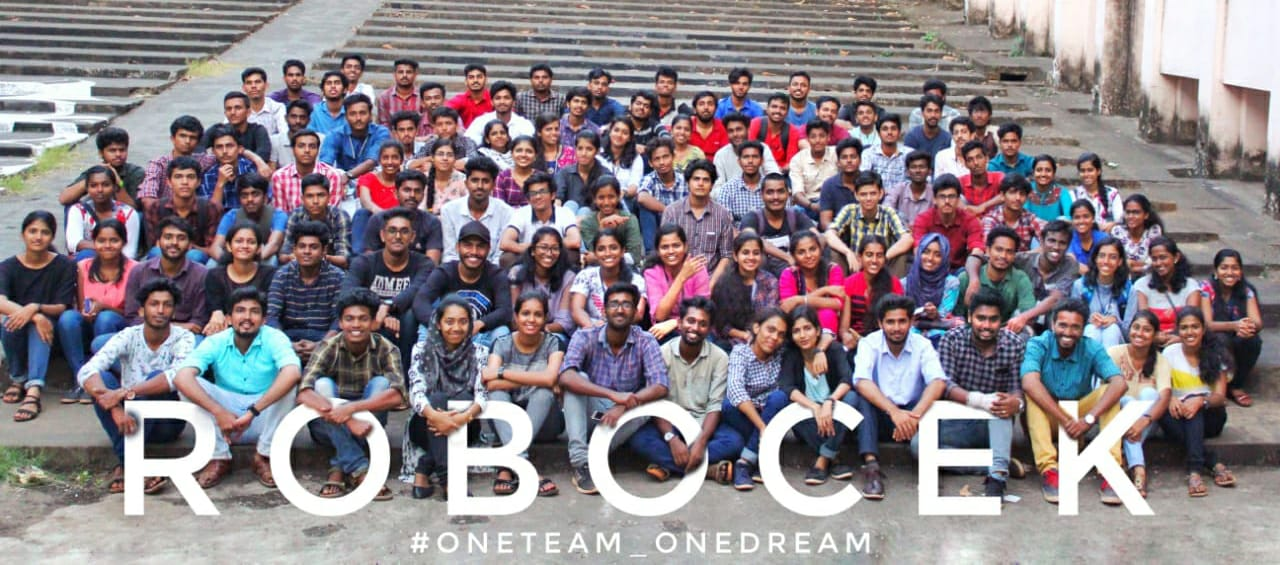
\includegraphics{Images/ROBOCEK/robocek.jpeg}
\end{figure}

\par ROBOCEK gradually evolved from a handful of members with no background in robotics into one of the most highly acclaimed robotics club in Kerala with a dedicated team and unmatched performance. The hardcore activities were accomplished by the students who organised themselves into an Executive Committee with prominent guidance from the Staff Advisors. They realised the dream of a room dedicated to ROBOCEK in GCEK. They conceived the idea of a basic workshop that would pave a path into the realm of robotics under ROBOCEK and finally converged to \textit{'ACTUATOR',The Beginner's Workshop}. Bit by bit 'Actuator' turned to be the first and the most interesting workshop that waved among the freshers of GCEK and also any entry point into the ROBOCEK. The pioneers into the club slowly engaged themselves into learning in groups.

The dedicated cluster of students strived to explore the intangible sphere of robotics through workshops, competitions, collaborative learning and expeditions nurturing academic excellence striving to keep in pace with electronics and robotics. The team endeavoured various tech fests, including national level fest - Xplore'19 and social relevant projects like expo's,flood relief activities, workshops etc.

\section{ROBOCEK Execom}
    \begin{figure*}
        \centering
        \subfloat{
\includegraphics[width=2.7in]{Images/ROBOCEK/execom_2020_21.jpeg}}\quad
        \subfloat{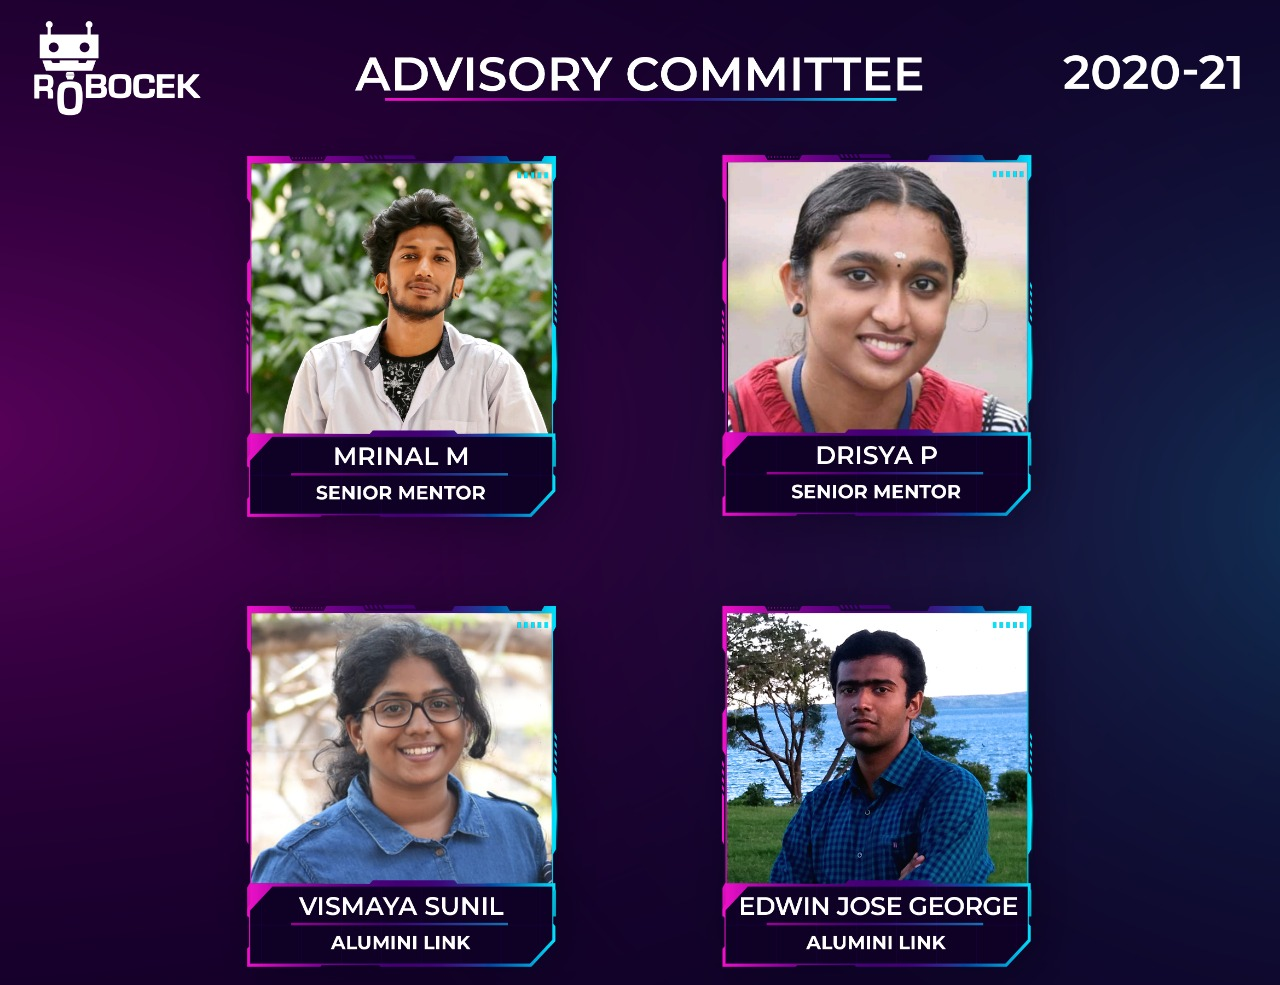
\includegraphics[width=2.7in]{Images/ROBOCEK/Advisory_Committee_2020.jpeg}}
    \end{figure*}
    
    \begin{figure*}
        \centering
        \subfloat{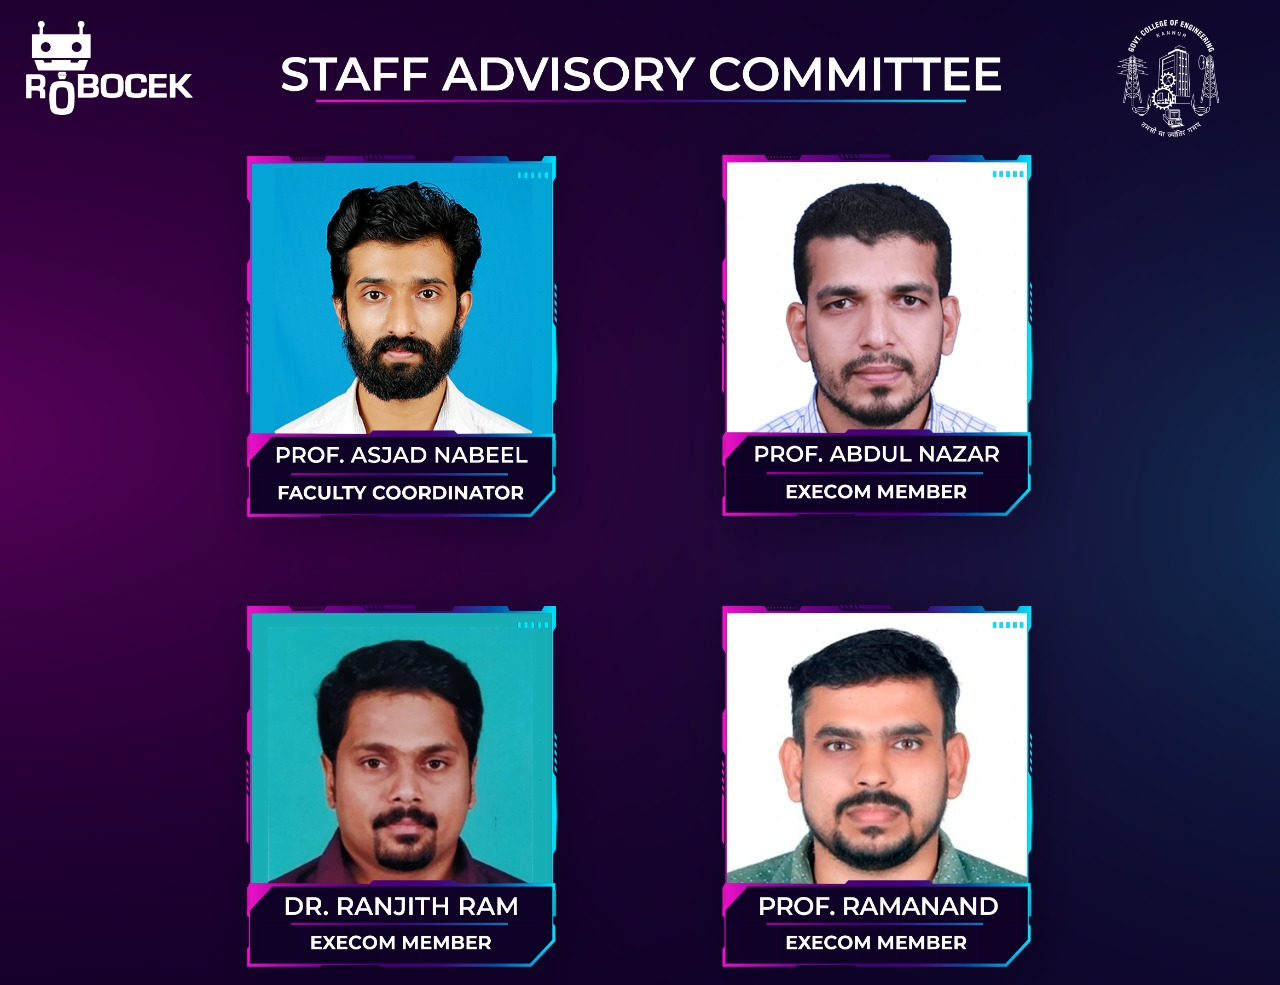
\includegraphics[width=2.7in]{Images/ROBOCEK/staff_advisors.jpeg}} \\
        \subfloat{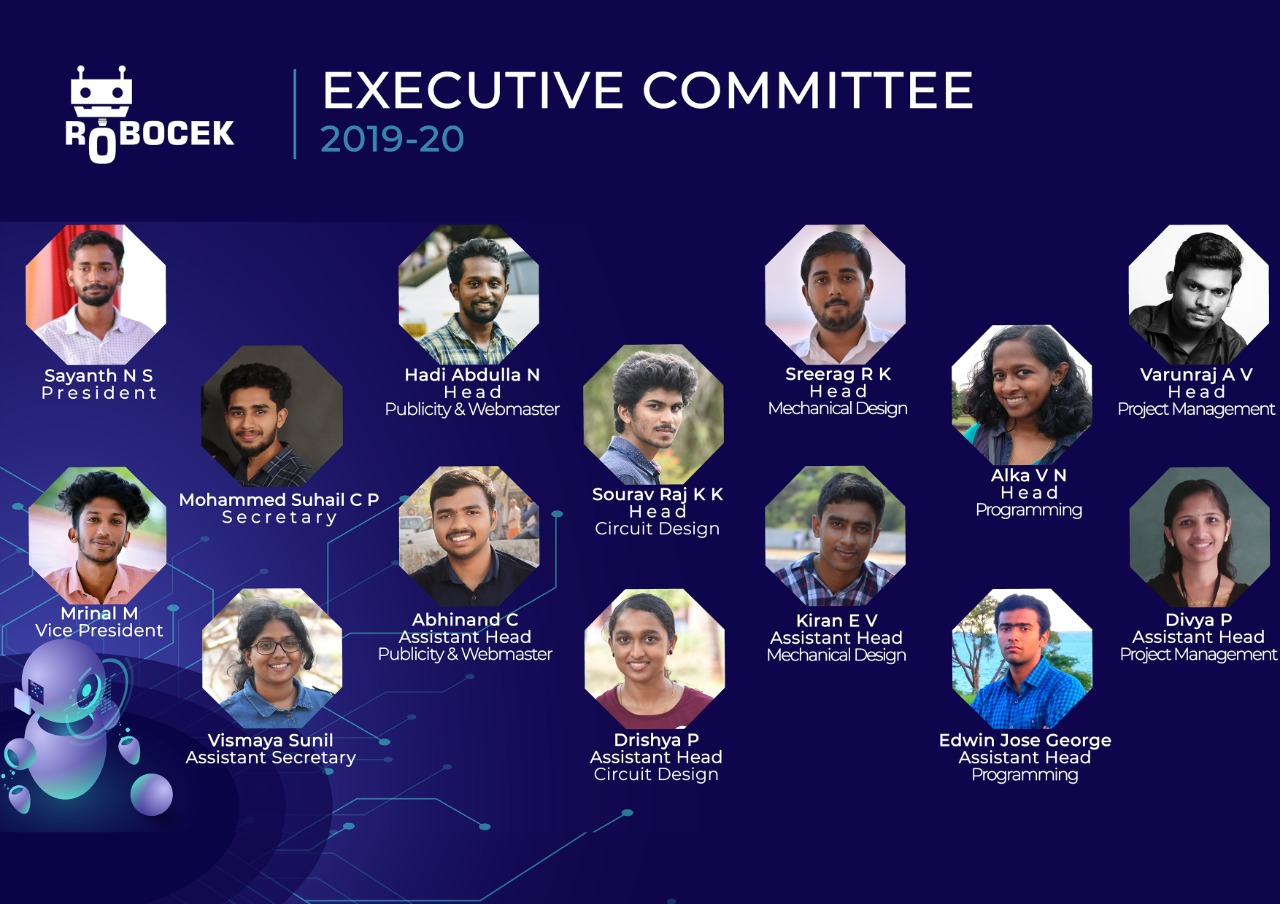
\includegraphics[width=2.7in]{Images/ROBOCEK/execome_2019_20.jpeg}}\quad
        \subfloat{
\includegraphics[width=2.7in]{Images/ROBOCEK/execom_2017_18.jpeg}}
    \end{figure*}
    
    Its always been a proud moment to see an enthusiastic team that shape the progress of our club. Starting from 2014, <name> layed the foundation for the robotics club for the first time in GCE Kannur. Lead by <name>, striving through initial and difficult times, along with support from faculty, we payed a better way for the future generation of the college to invest their interest and passion in technology. With rising demand for betterment, an excellent team of enthusiastic students were chosen to drive ROBOCEK, meeting the vision and mission of the club. Though lead by a team, each and every innovations are always welcomed, helping the students to advance their career. Our courage to advance is the everlasting support from ROBOCEK Alumni, providing with examples and support for aspirants.

\newpage
\section{Reach out to us}
\begin{table}
\centering
    \begin{tabular}{ll}
    \ci{\faIcon{globe}}    & \url{https://robocek.org/}                            \\
    \ci{\faIcon{envelope}}  & \href{mailto: robocek@gcek.ac.in}{robocek@gcek.ac.in} \\
    \ci{\faIcon{envelope}}  & \href{mailto: robocek@gmail.com}{robocek@gmail.com} \\
    \ci{\faIcon{github}}    & \url{https://github.com/robocek} \\
    \ci{\faIcon{linkedin}}  & \url{https://www.linkedin.com/company/robocek/}       \\
    \ci{\faIcon{facebook}}  & \url{https://www.facebook.com/robocek/}               \\
    \ci{\faIcon{instagram}} & \url{https://www.instagram.com/robocek\_official/}      \\
    \ci{\faIcon{youtube}}   & \url{https://www.youtube.com/ROBOCEK}
    \end{tabular}
\end{table}

%----------------------------------------------------------------------------------------
%	CHAPTER 1 : Introduction to Robotics
%----------------------------------------------------------------------------------------
\chapter{Introduction to Robotics}
%------------------------------------------------

\section{What is Robotics?}
\par Robotics is an interdisciplinary field that integrates Computer Science and Engineering. It comprises design, construction, operation and use of robots. The field targets the creation of machines that can help and assist humans through blending aspects of mechanical engineering, electrical engineering, mechatronics, electronics etc
\par A Robot is an interactive machine capable of carrying out a complex series of actions automatically, especially one programmable by a computer, to reduce human risk in hazardous works. Thus, robotics is an interdisciplinary branch of engineering and science that deals with the design, construction, operation, and use of robots, as well as computer systems for their control, sensory feedback, and information processing to create an efficient robot. A robot can be thought as an combination of sensors, controllers and actuators. Sensor provide collection of information from environment, that are processed by controllers who generate signal to actuators to interact with environment.
\par Robots are put to use in different applications. Their usage is determined by the field they concentrate on. Robotics is a vast field. They may be manufactured or processed in different forms, shapes and utility. Joseph Engelberger, godfather of robotics, once said \textit{“I can't define a robot, but I know one when I see one.”}

\section{Evolution of Robotics}
\par The question of evolution of robotics take us to the ancient world and era of industrial revolution. Engineers were trying to develop machines that can handle dangerous tasks for automotive industry and defence. Robots they developed were meant to be a replica of human actions. 
\begin{table*}
    \centering
    \begin{tabular}{|c|p{14cm}|}
    \hline
        \textbf{\textit{Year}} & \hspace{30mm}\textbf{\textit{Major Events in History of Robotics}} \\ \hline
        
        \rowcolor[gray]{0.95} 1801 & Joseph Jacquard builds an automated loom that is controlled by a punch card. Punch cards are later used as an input method for some early 20th century computers. \\ \hline
        
        1921 & Writer Karel Capek introduced the term \textbf{'robot'} in his play 'Rossum's Universal Robots'. The word \textbf{'robot'} evolved from the word 'robota' meaning 'work'. \\ \hline
        
        \rowcolor[gray]{0.95} 1941 & Developed from the idea by Karel Capek, Science Fiction Writer Isaac Asimov first used the word \textbf{'robotics'} to describe the technology of robots. \\ \hline
        
        1942 & Isaac Asimov wrote the \textbf{'Three Laws of Robotics'} which is still considered as the foundational rules of robotic industry. \\ \hline
        
        \rowcolor[gray]{0.95} 1950 - 60 & The first ever industrial robot \textbf{Unimate} was designed by George Devol and Joe Engelberger. The 4,000-pound robot arm sequenced and stacked hot pieces of die-cast metal. \\ \hline
        
        1969 & Victor Scheinman designed a \textbf{Stanford arm} which eventually became a standard and is still influencing the design of robotic arms today. \\ \hline
        
        \rowcolor[gray]{0.95} 1974 & \textbf{IRB-6}, the first electric industrial robot that was controlled by a microcomputer. The major features were that it was programmable, had 16KB of RAM, and display four whole digits with LEDs. \\ \hline
        
        1986 & Honda introduced a \textbf{Robot Research Program} which came up with ideas that a robot should coexist and cooperate with human beings. \\ \hline
        
        \rowcolor[gray]{0.95} 1977 & The NASA \textbf{Pathfinder Mission} lands on Mars. Its robotic rover Sojourner broadcasts data from Martian surface. \\ \hline
        
        1999 & The Sony \textbf{Aibo} offers users a robotic pet dog with learning and communication potential. Aibo christens a revolutionary drive in consumer robotics and technology with more affordable iterations appearing throughout the next decade. \\ \hline
        
        \rowcolor[gray]{0.95} 2005 &  Honda’s \textbf{Advanced Step in Innovative Mobility (ASIMO)} humanoid robot is introduced. It could walk 1 mph, climb stairs and change its direction after detecting hazards. Using the camera mounted in its head, ASIMO could also recognize faces, gestures and the movements of multiple objects. \\ \hline
        
        2016 & \textbf{Sophia}, a social Humanoid robot developed by Hong Kong-based company Hanson Robotics. It is the first humanoid to receive citizenship to a country. It has the unique ability to connect and communicate with humans in an unforgettable way, showcasing our unparalleled robotics art and design, AI science, and engineering.\\ \hline
        
    \end{tabular}
\end{table*}

%----------------------------------------------------------------------------------------
%	CHAPTER 2 : Introducing to Arduino
%----------------------------------------------------------------------------------------
\chapter{Introduction to Arduino}
\label{ch:arduino-uno}
\par Arduino is it one of the most widely used micro-controller to develop various DIY projects. The low cost and easy to deploy has given rise to various \ac{IoT} and embedded projects. Arduino is an open source electronics platform based on easy-to-use hardware and software. Usually the term “Arduino” can be used to refer the following.

\begin{itemize}
    \item Open Source Electronics Platform : Free to design and implement various units, easy availability and high customization. 
    \item Arduino \ac{IDE} : A software to program Arduino boards.
    \item Online Arduino Community : Fast growing community who maintains and supports Arduino Developments. \\
    \url{https://github.com/arduino/} \hspace{0.5cm} \url{https://www.arduino.cc/}

\end{itemize}

\par The Arduino project was started in 2005 as a program for students at the Interaction Design Institute Ivrea in Ivrea, Italy , aiming to provide a low-cost and easy way for novices and professionals to create devices that interact with their environment using sensors and actuators. The name Arduino comes from a bar in Ivrea, Italy, where some of the founders of the project used to meet. The ease at which various units can be attached gained Arduino its popularity. Anyone can start with programming and robotics by just following the step by step instructions of a kit, or sharing ideas online with other members of the Arduino community.

\par Following are few of the key points of Arduino :

\begin{itemize}
    \item Easy to use and expensive
    \item Cross-platform and open source
    \item Simple and clear programming
    
    \begin{marginfigure}
		
\includegraphics{Images/Intro_Arduino/arduino_community.png}
        \captionsetup{type=figure}
        \caption{\raggedright Arduino Open Source Community}
    \end{marginfigure} 
    
    \item  Extensible software/hardware
\end{itemize}   

\section{Comparing Arduino to its alternatives}
\par Arduino is not the only board available to build custom projects and applications. Raspberry Pi, BeagleBone, Sharks Cove, Minnowboard MAX, Nanode, Waspmote or LittleBits are some of the most interesting alternatives to Arduino. Arduino and Raspberry Pi are the ones receiving the most attention within the community of software developers.

\paragraph{ } Raspberry Pi is a low cost \ac{SBC} developed by the British Raspberry Pi Foundation. They are used in places which require higher and faster calculations. They are boards with micro processors. Raspberry Pi acts as a mini computer with additional I/O connection pins along with Wi-Fi, Bluetooth and ability to connect to external devices via HDMI, USB ports etc.. It have a complete Operating System (Raspberian) burned into a SD card. 

\paragraph{ } Arduino, on the other hand is a low cost \ac{SoC} board. They are used where complex information need not be analyzed. They are heavily used in Embedded systems and \ac{IoT}. They are boards with micro controller that control other appliances. There are no Operating System burned into Arduino. Arduino simply uses machine code to execute instructions. The machine code are created by compiling programs written in high level languages like C, into an executable binary file.

\begin{figure}
    \centering
    \subfloat[Arduino Uno R3]{
        \label{fig : arduino_uno_r3 } 
        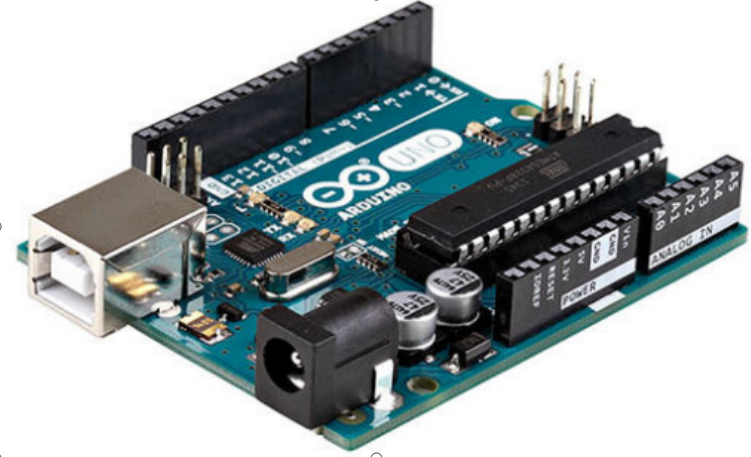
\includegraphics[width=2in]{Images/Intro_Arduino/arduino_uno.png}
    }
    \subfloat[Raspberry Pi 2 Model B]{
        \label{fig : raspberry_pi_2}
        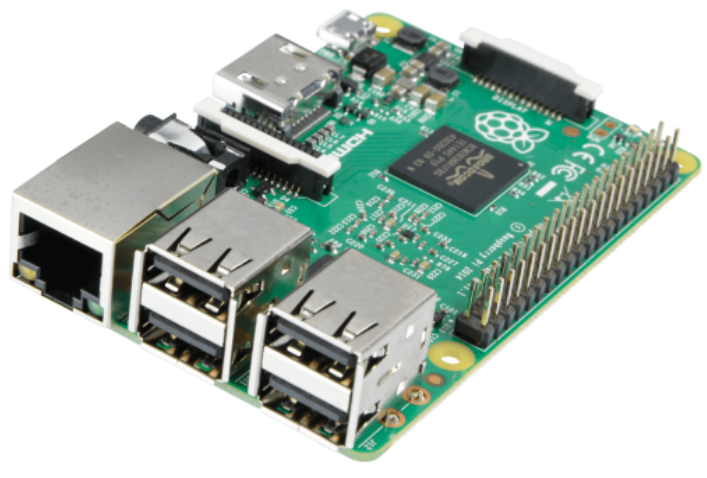
\includegraphics[width=2in]{Images/Intro_Arduino/raspberry.png}
    }
    \caption{Development boards}
\end{figure}

\section{Micro-controllers and Micro-processors}
Micro-controllers and Micro-processors are common terms used in \ac{IoT} and embedded systems. It is worth a while to understand the difference between them, to choose which is better to our project need.
\paragraph{ } Micro-controllers and micro-processors are used to execute instructions and control various units interfaced with them. However their complexity and utility can vary greatly. Micro controllers are similar to a small computer fabricated into a single \ac{IC}. It contains a processor core, ROM, RAM, and I/O pins It does not need any external circuits to do its task. It can manage memory and other services its own. It does the job of managing units as well an performing calculations. Micro-processor, on the other hand, has only CPU inside them. It does not have RAM, ROM of its own. Processors are dedicated to perform calculations. They depend on external circuits for its peripheral like RAM, ROM to work. They are used where the task are complex and tricky. The features are summarized in table \ref{tab:compare_micro_proc}.

\begin{figure}
    \centering
    \subfloat[Microprocessor]{
        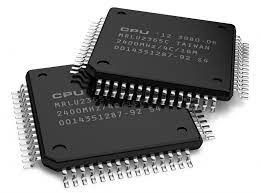
\includegraphics[width=1.2in]{Images/Intro_Arduino/processor.jpeg}
    }\qquad
    \subfloat[Micro-controller]{
        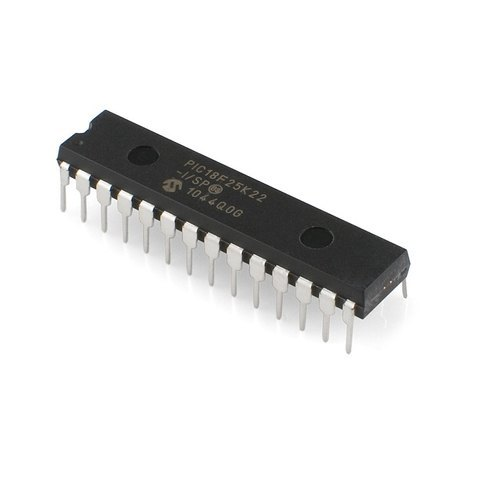
\includegraphics[width=1.2in]{Images/Intro_Arduino/microcontroller.jpg}
    }
    \caption{Processor and Micro-Controllers}
\end{figure}

\begin{table*}
    \renewcommand{\arraystretch}{1.5}
    \resizebox{5in}{!}{%
        \begin{tabular}{|l|l|}
        \hline
        \multicolumn{1}{|c|}{\textit{\textbf{Micro processor}}} &
          \multicolumn{1}{c|}{\textit{\textbf{Micro controller}}} \\ \hline
        RAM, ROM, EEPROM needs to be connected         & RAM, ROM, EEPROM are present on single IC \\ \hline
        Expensive                                      & Cheap                                     \\ \hline
        High processing speed (\textgreater{}1Ghz)     & Low processing speed (\textless{}50Mhz)   \\ \hline
        No power saving technology                     & Optimized power usage                     \\ \hline
        Used in large applications                     & Used in small application                 \\ \hline
        Process complex task                           & Process simple task                       \\ \hline
        Dissipate high heat. Might need cooling        & Does not dissipate high heats.            \\ \hline
        \begin{tabular}[c]{@{}l@{}}Usage of external storage\\ (HardDisk - GB of spaces)\end{tabular} &
          \begin{tabular}[c]{@{}l@{}}Usage of internal Storage\\ (EEPROM - few KB space)\end{tabular} \\ \hline
        Eg: Intel Pentium 4, Intel Core i7, AMD Athlon & Eg: ATmega328, ESP8266, ESP32, ATMEGA32U4 \\ \hline
        Board: Raspberry Pi                            & Board: Arduino                            \\ \hline
        \end{tabular}%
    }
    \vspace{0.5cm}
    \caption[Microprocessors VS Micro-controllers]{Comparison of Microprocessors and Micro-controllers}
    \label{tab:compare_micro_proc}
\end{table*}

\section{Arduino Boards}
Arduino is a large community that develops various micro-controller boards. Depending on the project application and usage, various customized official boards are available. The most generally used Arduino board is the “Arduino Uno”. We would be making use of Arduino Uno to develop various projects.

\begin{figure*}
  \centering
  \subfloat[Arduino Due]{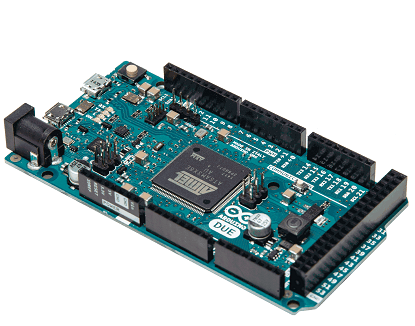
\includegraphics[width=2in]{Images/Intro_Arduino/ard_due.png}} \quad
  \subfloat[Arduino Leonardo]{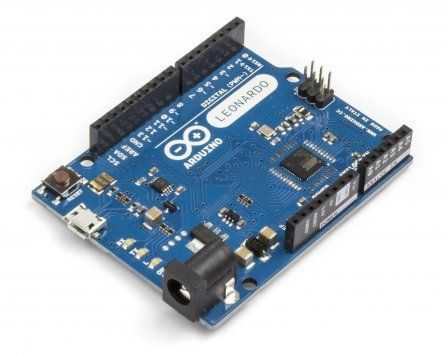
\includegraphics[width=2in]{Images/Intro_Arduino/ard_leonardo.jpg}}\quad
  \subfloat[Arduino Uno R3]{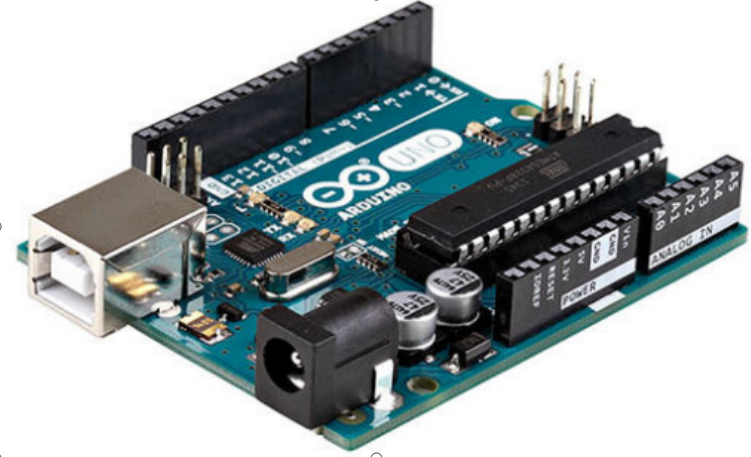
\includegraphics[width=2in]{Images/Intro_Arduino/arduino_uno.png}}\\
  \subfloat[Arduino Mega 2560]{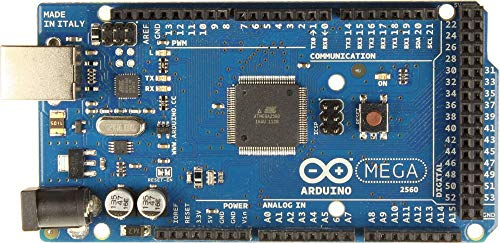
\includegraphics[width=2in]{Images/Intro_Arduino/ard_mega.jpg}}\quad
  \subfloat[Arduino Nano]{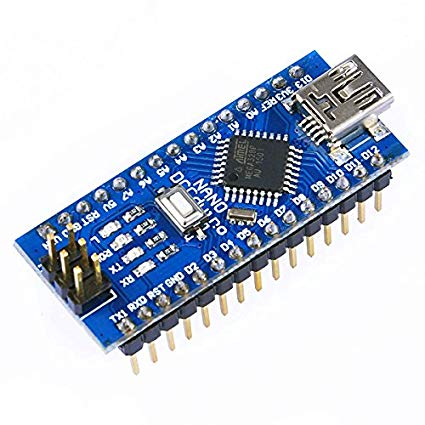
\includegraphics[width=2in]{Images/Intro_Arduino/ard_nano.jpg}}\quad
  \subfloat[LillyPad Arduino]{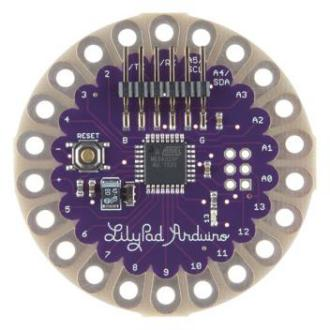
\includegraphics[width=2in]{Images/Intro_Arduino/ard_lillypad.jpg}}
  \caption{Arduino Boards}
\end{figure*}

\begin{figure}
    \centering
    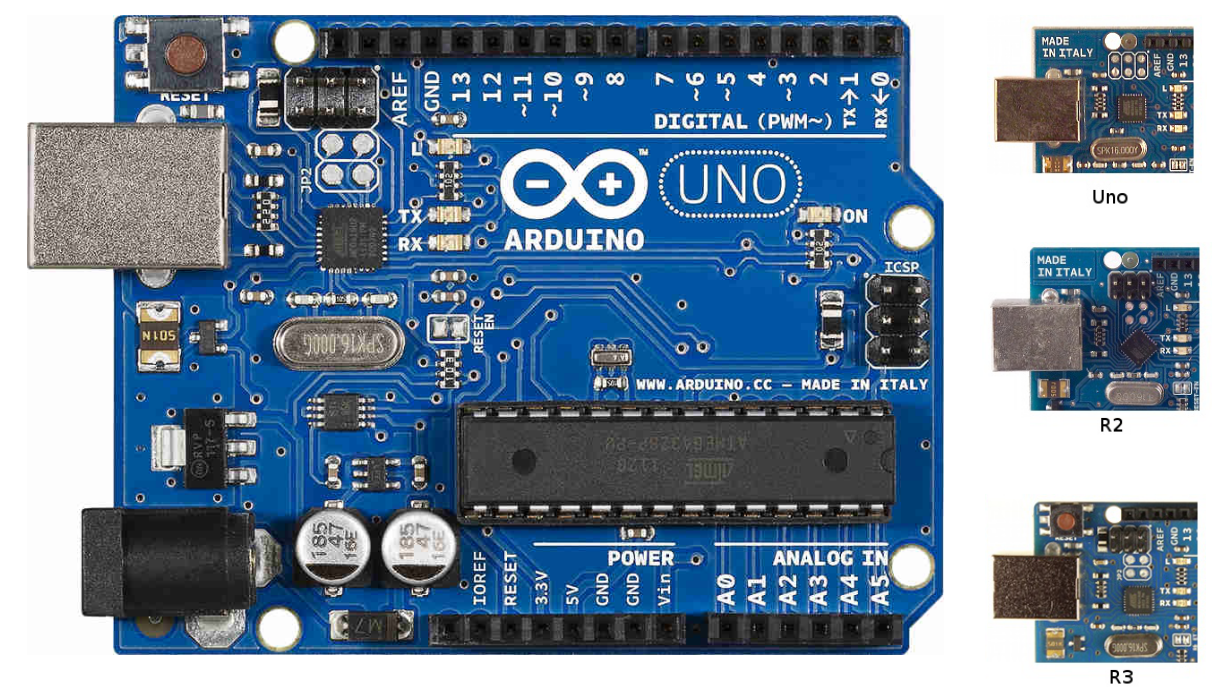
\includegraphics[width=4.3in]{Images/Intro_Arduino/arduino_uno_versions.png}
    \caption[Arduino Uno version]{Arduino Uno versions. Notice the alignment and position of ATMega16U2 micro-controller}
\end{figure}
\newpage

\section{Arduino Uno R3}
    \subsection{On-board units}
    
    \begin{figure}
        \centering
        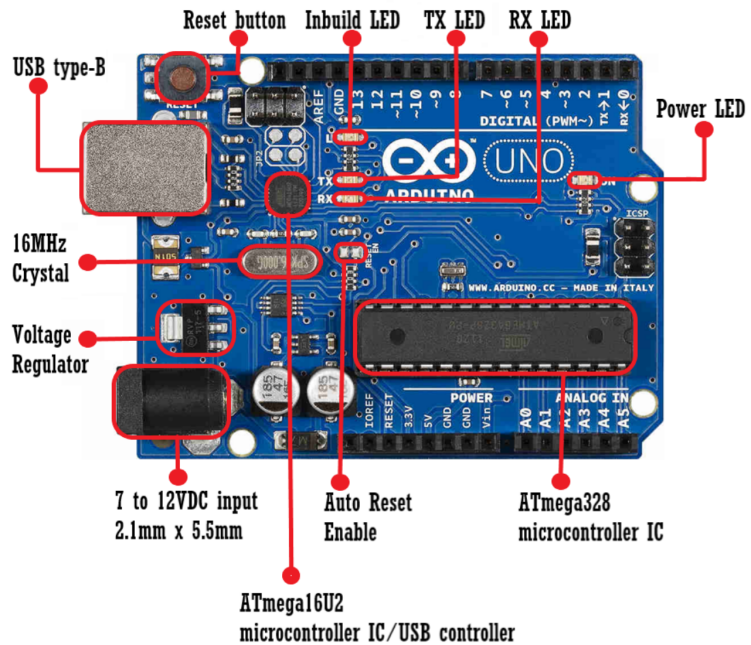
\includegraphics[width=\textwidth]{Images/Intro_Arduino/uno_desp.png}
        \caption{Arduino Uno R3 Pinout}
    \end{figure}
    
    \begin{itemize}
        \item ATmega328 micro controller \\
        Heart of Arduino Uno R3. This micro controller unit executes instructions. Programs are stored inside this unit.
        \item ATmega16U2 micro controller\\
        Used to assist main micro controller. Placed near to USB port to decode USB information. Stands as a boot loader that write programs into main micro controller. The transmit LED (Tx LED) and receive (Rx LED) turns on whenever read or write operations are performed to micro-controllers. 
        \item 16Mhz\\
        Act as heart beat of Arduino board. Serves as clock for timing various signals.
        \item Use type-B\\
        Used to interface Arduino to computer. Arduino board can be programmed via USB. Serial communication with board and serial monitor can also be achieved.
        \item 12V DC input\\
        The board can be powered via 12V DC adapter. The 12V is passed via capacitors to provide enough ampere and voltage across the board.
        \item Voltage regulator\\
        The digital circuits usually work at 5V. The 5V voltage regulator ensures that all the units gets proper voltage levels. If the board is successfully powered, the power LED glow brightly.
        \item Reset Button\\
        At time we might need to restart the board from the beginning. The reset button is used to reload the program from start. The reset can also be triggered inside the program.
    \end{itemize}
    
    \subsection{Micro controller : ATmega328}
    
    \begin{table}
        \centering
        \begin{tabular}{|l|l|}
            \hline
            \multicolumn{1}{|c|}{\textit{\textbf{Parameter}}} & \multicolumn{1}{c|}{\textit{\textbf{Value}}} \\ \hline
            CPU Type                    & 8-bit AVR       \\ \hline
            Performance                 & 20MIPS at 20MHz \\ \hline
            Flash Memory                & 32 KB           \\ \hline
            SRAM                        & 2 KB            \\ \hline
            EEPROM                      & 1 KB            \\ \hline
            Pin Count                   & 28 or 32 pins   \\ \hline
            Maximum operating frequency & 20Mhz           \\ \hline
            Maximum I/O pins            & 23              \\ \hline
            External Interrupts         & 2               \\ \hline
            Board: Raspberry Pi         & Board: Arduino  \\ \hline
        \end{tabular}
        \caption{ATmega328 spec}
    \end{table}

\section{Pin Layout}
Pins of Arduino can be broadly divided into two categories depending on their utility. For each pin, there is a marking on the board to denote the function of that pin. Pins are divided into:
\begin{enumerate}
    \item General Purpose Input Output pins ( total 20 pins )\\ 
    The functions of these pins can be programmed as per user need. They can either act as input pins or output pins. Input pins are those pins which Arduino would be listening for voltage variations. Output pins are those pins where Arduino controls the output voltage. These pins can also be classified into two categories. They are 
    \begin{itemize}
        \item Digital Pins
        \item Analog Pins
    \end{itemize}
    
    \item Special Purpose pins (total 9 pins)\\
    The functions of these pins are predetermined and cannot be changed. They are reserved for special purpose. They include VCC (5v and 3.3v) , Vin, GND, RESET, IOREF, AREF, ICSP header.
    
    \par VCC pins provide a fixed output voltage, acting as a positive terminal of a cell. GND pin provide a fixed zero voltage. They act as the negative terminal of a cell. Any additional components that need to be interfaced with Arduino would surely be connected to GND pin. Vin pin is used to power up the Arduino. Depending on how the board is powered, Vin pin can also act as 5v VCC pin.
    \par RESET pin have the function similar to RESET push button. They can cause the program to restart from the beginning. IOREF and AREF stands for Input-output reference and Analog reference pin. They stand as a reference point to calculate voltages at digital and Analog pins. \ac{ICSP} header pins are place close to micro-controllers. It is the ability of a micro-controller to be programmed without disconnecting from the circuitry.
\end{enumerate}

\section{Methods to power up Arduino}
There are mainly three ways to power up the board. 
\par The first method is to use UBS cable to power up the device. Just connect USB port to computer or a power bank. In this method the Vin pin can act as a 5V output pin. Make sure you don’t draw much power so as the damage the port. The 12V DC jack should be kept free. 
\par The second method is the power up via 12V DC jack. This will cause the board to have a bit higher current to handle components connect to it. The Vin pin act as a constant 5V DC output pin. In this method the USB port should to kept free. To make serial communication, make use of pins 0,1. 
\par The third pin is to power 5V via Vin pin. The 12V jack and USB must be kept free. In this method, the board is likely to run on lower ampere.

\section{Digital Pins}
\par Digital pins are those pins that act on digital values. A positive 5V (above 2.5V) act as binary 1 or HIGH digital signal. A ground 0V (below 2.3V) act as binary 0 or LOW digital signal. Arduino being a digital system, all general purpose input-output pins can be used as digital pins. There are total of 20 pins that can be used for digital signals, ranging from pin 0 to pin13 and A0 to A5. To make use of digital signals we make use of functions like digitalRead() and digitalWrite().

\begin{figure}
 \centering
 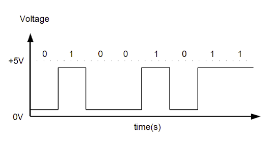
\includegraphics[width=3.5in]{Images/Intro_Arduino/digital_graph.png}
 \caption{Digital signals}
\end{figure}

\section{Analog Pins}
\par The pins that support analog input are called analog pins. Analog signals are those signals that vary continuously. That is, they do not have a specific cutoff like digital signals. They can assume wide range of values. Temperature is an example of analog signals that vary continuously. Since Arduino is an digital circuit, the analog signals needs to be converted to digital signals for the micro controller to understand. This function is performed by \ac{ADC}. \ac{ADC} convert analog signal to 10bit digital value by sampling the signal and then mapping each sample to $2^{10}$ levels. There are a total of 6 pins in Arduino Uno that supports \ac{ADC}, ranging from pins A0 to A5. To read analog value we make use of function analogRead().

\begin{figure}
 \centering
 \includegraphics[width=\textwidth]{Images/Intro_Arduino/analog_graph.png}
 \caption{Analog signals}
\end{figure}

\section{\ac{PWM}}
\ac{PWM} is the technique used to convert the digital signals to analog output results from Arduino. Arduino cannot directly produce various voltage levels. Being a digital circuit, it can only produce voltage levels 0V and 5V. To stimulate an analog effect, it creates square waves. The square wave have two key components: frequency and duty cycle. Frequency stays constant of about 500 Hz whereas the duty cycle is manipulated. Duty cycle refers to the amount of time signal stays high in a given time cycle. If Duty cycle is 100\%, we would get an effect of 100\% of 5V = 5V. If Duty cycle is 50\%, we would get an effect of 50\% of 5V = 2.5V. 

\par Arduino Uno can support \ac{PWM} on its 6 selected pins. They are pins 3, 5, 6, 9, 10 and 11. These pins have a tilde symbol ( \textasciitilde{} ) associated with their pin number on the board. The analog output function accepts 8 bit numbers, that are mapped to duty cycle. The 8 bit numbers can produce $2^8=256$ possible variations, spanning from zero to 255. The function analogWrite() is used to  produce analog output from Arduino at \ac{PWM} pins.

\begin{figure}
 \centering 
 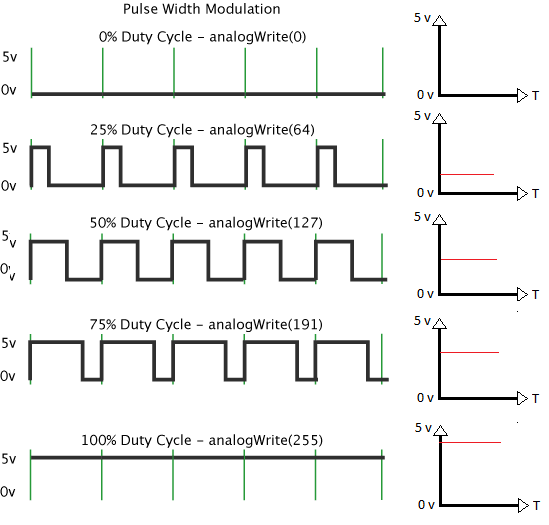
\includegraphics[width=3.5in]{Images/Intro_Arduino/pwm.png}
 \caption{Pulse width Modulation}
\end{figure}

\renewcommand{\arraystretch}{1.2}
\begin{table}
	\raggedright
    \resizebox{\textwidth}{!}{%
        \begin{tabular}{|l|l|}
        \hline
        \multicolumn{1}{|c|}{\textit{\textbf{ADC}}} & \multicolumn{1}{c|}{\textit{\textbf{PWM}}} \\ \hline
        Analog to Digital Converter                 & Pulse Width Modulation                     \\ \hline
        \begin{tabular}[c]{@{}l@{}}Implements sampling on analog \\ signals to convert to digital values\end{tabular} &
          \begin{tabular}[c]{@{}l@{}}Uses width of the pulse ( duty cycle) to \\ convert digital to analog signals\end{tabular} \\ \hline
        10 bit resolution : input                   & 8 bit resolution : output                  \\ \hline
        Applicable only on A0 to A5                 & Applicable only on 3, 5, 6, 9, 10, 11      \\ \hline
        analogRead()                                & analogWrite()                              \\ \hline
        \end{tabular}%
    }
    \caption{ADC v/s PWM}
\end{table}
\renewcommand{\arraystretch}{1}

\newpage
\begin{figure*}
    \centering
    \includegraphics[height=8.25in]{Images/Intro_Arduino/datasheet.png}
    \caption{Arduino Uno Data-sheet}
\end{figure*}











%----------------------------------------------------------------------------------------
%	CHAPTER 3 : Programming Arduino
%----------------------------------------------------------------------------------------
\chapter{C Programming on Arduino Uno}
%------------------------------------------------

\section{Session 1}
This is a bunch of session content. This is a bunch of session content. This is a bunch of session content. This is a bunch of session content. This is a bunch of session content. This is a bunch of session content. This is a bunch of session content. This is a bunch of session content. This is a bunch of session content. This is a bunch of session content. This is a bunch of session content. This is a bunch of session content. This is a bunch of session content. This is a bunch of session content. This is a bunch of session content. This is a bunch of session content. This is a bunch of session content. This is a bunch of session content. This is a bunch of session content. This is a bunch of session content. This is a bunch of session content. This is a bunch of session content. This is a bunch of session content. This is a bunch of session content. This is a bunch of session content. This is a bunch of session content. This is a bunch of session content. This is a bunch of session content. This is a bunch of session content. This is a bunch of session content. This is a bunch of session content. This is a bunch of session content.
%------------------------------------------------

\section{Session 2}
This is a bunch of session content. This is a bunch of session content. This is a bunch of session content. This is a bunch of session content. This is a bunch of session content. This is a bunch of session content. This is a bunch of session content. This is a bunch of session content. This is a bunch of session content. This is a bunch of session content.
\paragraph{Paragraph1}
This is a paragraph content. This is a paragraph content. This is a paragraph content. This is a paragraph content. This is a paragraph content. This is a paragraph content. This is a paragraph content. This is a paragraph content. This is a paragraph content. This is a paragraph content. This is a paragraph content. This is a paragraph content. This is a paragraph content. This is a paragraph content. This is a paragraph content.
\paragraph{Paragraph2}
This is a paragraph content. This is a paragraph content. This is a paragraph content. This is a paragraph content. This is a paragraph content. This is a paragraph content. This is a paragraph content. This is a paragraph content. This is a paragraph content. This is a paragraph content. This is a paragraph content. This is a paragraph content. This is a paragraph content. This is a paragraph content. This is a paragraph content.

\section{Session 3}
This is a bunch of session content. This is a bunch of session content. This is a bunch of session content. This is a bunch of session content. This is a bunch of session content. This is a bunch of session content. This is a bunch of session content. This is a bunch of session content. This is a bunch of session content. This is a bunch of session content. This is a bunch of session content. This is a bunch of session content. This is a bunch of session content. This is a bunch of session content. This is a bunch of session content. This is a bunch of session content. This is a bunch of session content. This is a bunch of session content. This is a bunch of session content. This is a bunch of session content. This is a bunch of session content. This is a bunch of session content. This is a bunch of session content. This is a bunch of session content. This is a bunch of session content. This is a bunch of session content. This is a bunch of session content. This is a bunch of session content. This is a bunch of session content. This is a bunch of session content. This is a bunch of session content. This is a bunch of session content.


%----------------------------------------------------------------------------------------
%	CHAPTER 4 : Motor Driver
%----------------------------------------------------------------------------------------
\chapter{Motor Driver}
\label{chap:Motor_Driver}
%------------------------------------------------

\par As the name suggests, motor drivers are used to drive the motors. Motors consume higher current, more that what Arduino can supply. Hence they are interfaced with Arduino board using a motor driver. The motor driver consumes the power from external source and direct them to motors, controlled by Arduino. There are various motor drivers available. You might also able to find Arduino shields for motor drivers. A motor driver shield is much more powerful motor driver that can handle various DC motors, stepper motors, servo motors. In this session we would be talking about a simple motor driver - L298N

\begin{marginfigure}
\centering
  % include first image
  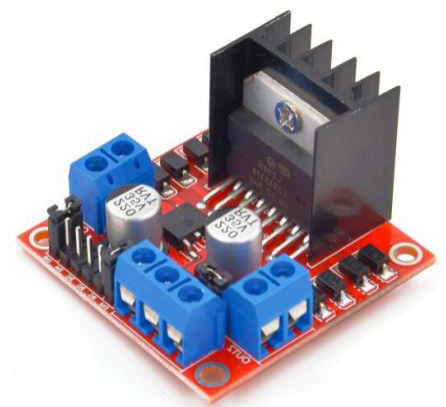
\includegraphics[width=.8\linewidth]{Chapters/images/MotorDriver_board.png}  
  \caption{Put your sub-caption here}
  
\end{marginfigure}

\begin{marginfigure}
\centering
  % include first image
  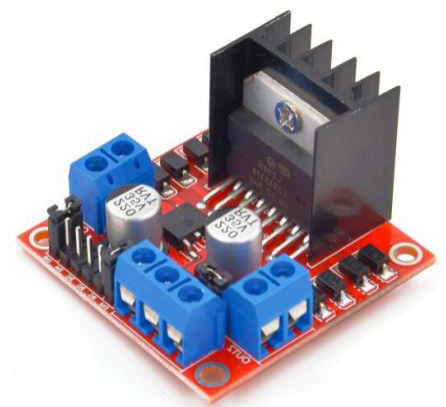
\includegraphics[width=.8\linewidth]{Chapters/images/MotorDriver_board.png}  
  \caption{Put your sub-caption here}
  
\end{marginfigure}
\section{L289N motor driver}
L298N motor driver is one of the many motor drivers available in the market. This driver have 4 out lines grouped into two as channel A and channel B. The working of the board is simple. Connect the external power source ( ~12V) to the +12V pin and the negative terminal of the source to the GND pin. Since we need to interface it with Arduino, we need connect the GND pin of Arduino to the GND pin of the board. The logical signals are supplied from Arduino to the board on the pins input1 to input4. When any of the logical pins are high, corresponding OUT pin turns on and gives an output of 10V. For example, if input3 is turned to HIGH, OUT3 would provide 10V and if input 2 is LOW, OUT2 would be at zero volt. \\
\begin{figure}
    \centering
    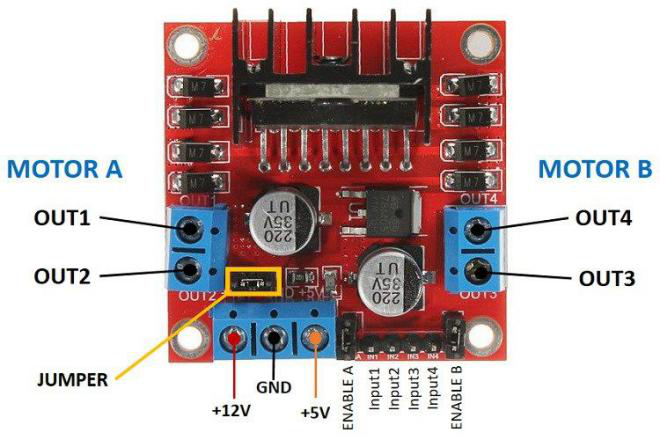
\includegraphics[width=2in]{Chapters/images/MotorDriver_desp.png}
    \caption{MotorDriver Description}
    \setfloatalignment{b}
\end{figure}
We can also find three jumper settings on the board. The jumper just above the power source (12V) connects the 5V pin via 5V regulator. The 5V pin is used to power IC on board. If the external power source is about 10 to 12 volts, we can keep this jumper on to power the board and motors using the 12V input. At this time, the 5V pin can act as an 5V output pin and can be used to power up the Arduino board. If we are providing external power supply greater than 12V, remove the jumper settings. The 5V regulator can get damaged. At this time, we would require additional 5V supply from Arduino to power the IC. L298N can handle up-to 35volts of external supply. Keep in mind that the board draws higher current and can exhaust your battery. Providing higher voltages can also cause the IC’s to heat up rapidly. Make sure to cool them if they crosses the threshold. \\
The second jumper you can find are at either sides of the logical input pins. On the left side we have jumper for channel A and on right side for channel B. These pins actually control the speed of the motors. To adjust the speed of motor in each channel, remove the jumpers and connect PWM pins of Arduino to control the speeds. If you want to function the motors at full capacity, keep the jumper ON.

\section{Interfacing DC motor - motor driver - Arduino}
\label{section:bot_interface}

Let us connect the motor driver and Arduino. The driver would be powered up via external supply and Arduino will be powered via USB cable. In this sample connection, lets connect and 10V DC motor to each channels. The next question is, how to control the direction of the motors? Lets consider the channel A. The terminal of the motor is connected to the OUT pins.
\begin{figure}
    \centering
    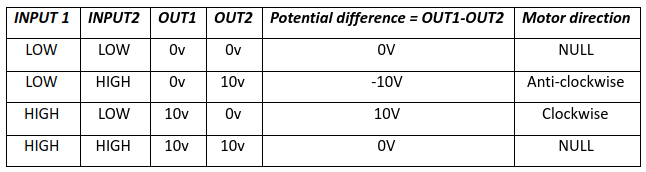
\includegraphics{Chapters/images/md1.png}
\end{figure}
\\ From the table below, it is clear that by inverting the logical signals, we can change the direction of motor. The same can be applied at the channel B for direction control. Now lets make the connections!

\begin{figure}
    \centering
    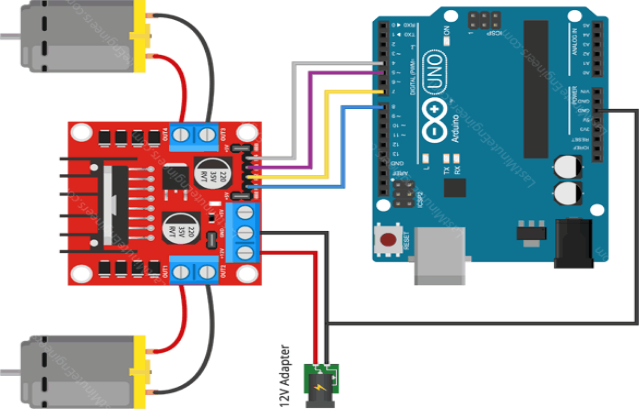
\includegraphics[width=2in]{Chapters/images/MotorDriver_circuit1.png}
    \caption{Interfacing MotorDriver with Arduino}
    \setfloatalignment{b}
\end{figure}

As shown in the figure, we have connected pins 8, 7, 5, 4 to input1, input2, input3 and input4 respectively. Both the boards shares the common GND and the driver is powered via 12V supply. Let’s write a program that turns the motors clockwise and anti clockwise to control the bot movement.\\

Code\\
\begin{lstlisting}[style=CStyle]
int m1 = 8, m2 = 7;  //left  motor pins
int m3 = 5, m4 = 4;  //right motor pins

void setup(){
//set motor pins as output for Arduino.
pinMode(m1,OUTPUT); pinMode(m2,OUTPUT);
pinMode(m3,OUTPUT); pinMode(m4,OUTPUT);
Serial.begin(9600);
}

//A function to control motor movement
void turn_motor(int input1, int input2, char dir){
if( dir == 'F'){
//clockwise rotation
digitalWrite(input1,HIGH);
digitalWrite(input2,LOW);
}
else if( dir == 'B'){
//anti-clockwise rotation
digitalWrite(input1,LOW);
digitalWrite(input2,HIGH);
}
else if( dir == 'S'){
//no rotation
digitalWrite(input1,LOW);
digitalWrite(input2,LOW);
}
}

void loop(){

turn_motor(m1, m2, 'F');  //left  wheel : clockwise
turn_motor(m3, m4, 'F');  //right wheel : clockwise
Serial.println("Bot moving forward");
delay(1000);

turn_motor(m1, m2, 'B');  //left  wheel : anti-clockwise
turn_motor(m3, m4, 'F');  //right wheel : clockwise
Serial.println("Bot turning left (rapidly)");
delay(500);

turn_motor(m1, m2, 'F');  //left  wheel : clockwise
turn_motor(m3, m4, 'B');  //right wheel : anti-clockwise
Serial.println("Bot turning right (rapidly)");
delay(500);

turn_motor(m1, m2, 'B');  //left  wheel : anti-clockwise
turn_motor(m3, m4, 'B');  //right wheel : anti-clockwise
Serial.println("Bot moving backward");
delay(1000);

turn_motor(m1, m2, 'S');  //left  wheel : stop
turn_motor(m3, m4, 'S');  //right wheel : stop
Serial.println("Bot stopped");
delay(5000);
}

\end{lstlisting}

Let’s summarize the bot movement of the above program.\\
\begin{figure}
    \centering
    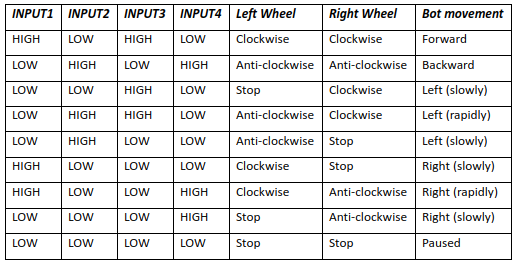
\includegraphics{Chapters/images/md2.png}
\end{figure} \\
You might have noticed that the bot drifts or becomes unstable when it changes it direction suddenly. This is because the wheels are rotating with higher speed than our bot can handle. The solution to such problems is the control the speed of the wheels. This can be easily achieved by making use of PWM pins in the motor driver. Lets try out our new speed controlled bot. It is easy to modify the above circuit and code to build the new bot quickly.

\section{Speed controlled Bot}
Re-configure the circuit by removing the jumper pins of channel A and B. Connect PWM pins 9 and 3 of Arduino to channel A and channel B respectively. You can identify PWM pins in Arduino by noticing the tilde symbol ( ~ ) on the board. The new circuit might look like this.
\begin{figure}
    \centering
    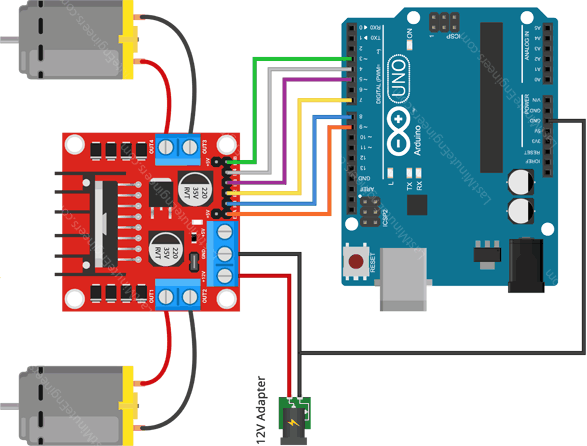
\includegraphics[width=2in]{Chapters/images/MotorDriver_circuit2.png}
    \caption{Interfacing Motors}
    \setfloatalignment{b}
\end{figure} \\
Now lets reconfigure the program \\
Code\\
\begin{lstlisting}[style=CStyle]
int pwmL = 9, m1 = 8, m2 = 7;  //left  motor pins
int pwmR = 3, m3 = 5, m4 = 4;  //right motor pins

void setup(){
//set motor pins as output for Arduino.
pinMode(m1,OUTPUT); pinMode(m2,OUTPUT); pinMode(pwmL,OUTPUT);
pinMode(m3,OUTPUT); pinMode(m4,OUTPUT); pinMode(pwmR,OUTPUT);
Serial.begin(9600);
}

//A function to control motor movement with speed regulation
void turn_motor(int input1, int input2, int speed_pin, int speed, char dir){
//Setting the speed
analogWrite(speed_pin, speed);

if( dir == 'F'){			//clockwise rotation
digitalWrite(input1,HIGH);
digitalWrite(input2,LOW);
}
else if( dir == 'B'){	//anti-clockwise rotation
digitalWrite(input1,LOW);
digitalWrite(input2,HIGH);
}
else if( dir == 'S'){	//no rotation
digitalWrite(input1,LOW);
digitalWrite(input2,LOW);
}
}

void loop(){

turn_motor(m1, m2, pwmL, 255, 'F');  //left  wheel : clockwise, speed=100%
turn_motor(m3, m4, pwmR, 127, 'F');  //right wheel : clockwise, speed=50%
Serial.println("Bot moving forward with small right curve");
delay(1000);

turn_motor(m1, m2, pwmL, 0, 'F');    //left  wheel : clockwise, speed=0%
turn_motor(m3, m4, pwmR, 127, 'F');  //right wheel : clockwise, speed=50%
Serial.println("Bot moving left with low speed");
delay(1000);
}

\end{lstlisting}
Keep in mind that PWM pins are 8-bit support pins. The Maximum analog value we can send is 255 i.e., $ 2^8 - 1 $ [ counting starts from zero ]. If PWM value is set to 255, the motors will run at full capacity and would decrease as the value decreases. Do note that you are controlling the effective voltage sent to the motor and not the actual wheel rotation. To control the rotation of the wheel precisely, we would have to make use of stepper motors.
\begin{figure}
    \centering
    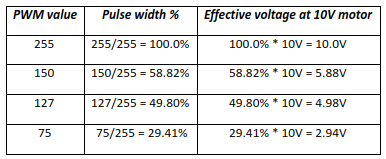
\includegraphics{Chapters/images/md3.png}
\end{figure}
Try connecting few sensors like Ultrasonic sensors, IR sensor, LDR, Accelerometer etc to make your bot autonomous and attractive!
\begin{figure}
    \centering
    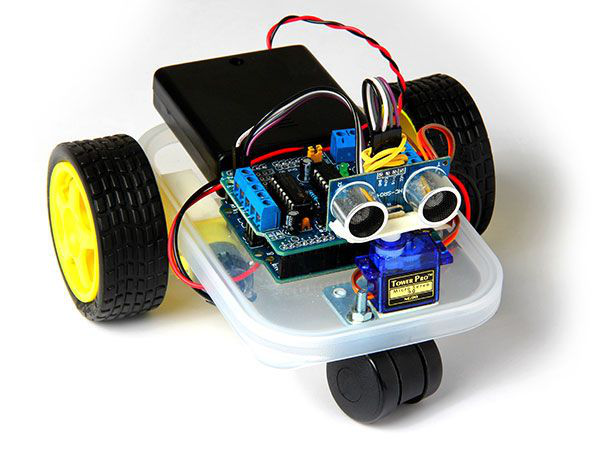
\includegraphics[width=3.2in]{Chapters/images/MotorDriver_end_pic.png}
    \caption{A Bot}
    \setfloatalignment{b}
\end{figure}
%----------------------------------------------------------------------------------------
%	CHAPTER 5 : Interfacing IR sensors
%----------------------------------------------------------------------------------------
\chapter{Interfacing IR sensors}
\label{ch:ir-sensors}
%------------------------------------------------

\ac{IR} stands for Infrared Radiation, is an \ac{EMR} with wavelengths longer than those of visible light. Discovered in 1800 by astronomer Sir William Herschel, \ac{IR} is a region of the \ac{EMR} spectrum where wavelengths range from about 700 nanometers (nm) to 1 millimeter (mm). They are longer than those of visible light, but shorter than those of radio waves. As they do not fall under the visible spectrum, they remain invisible to human eye. Certain animals and cameras can pick up those radiation and perceive them as images.

\begin{figure}
    \centering
	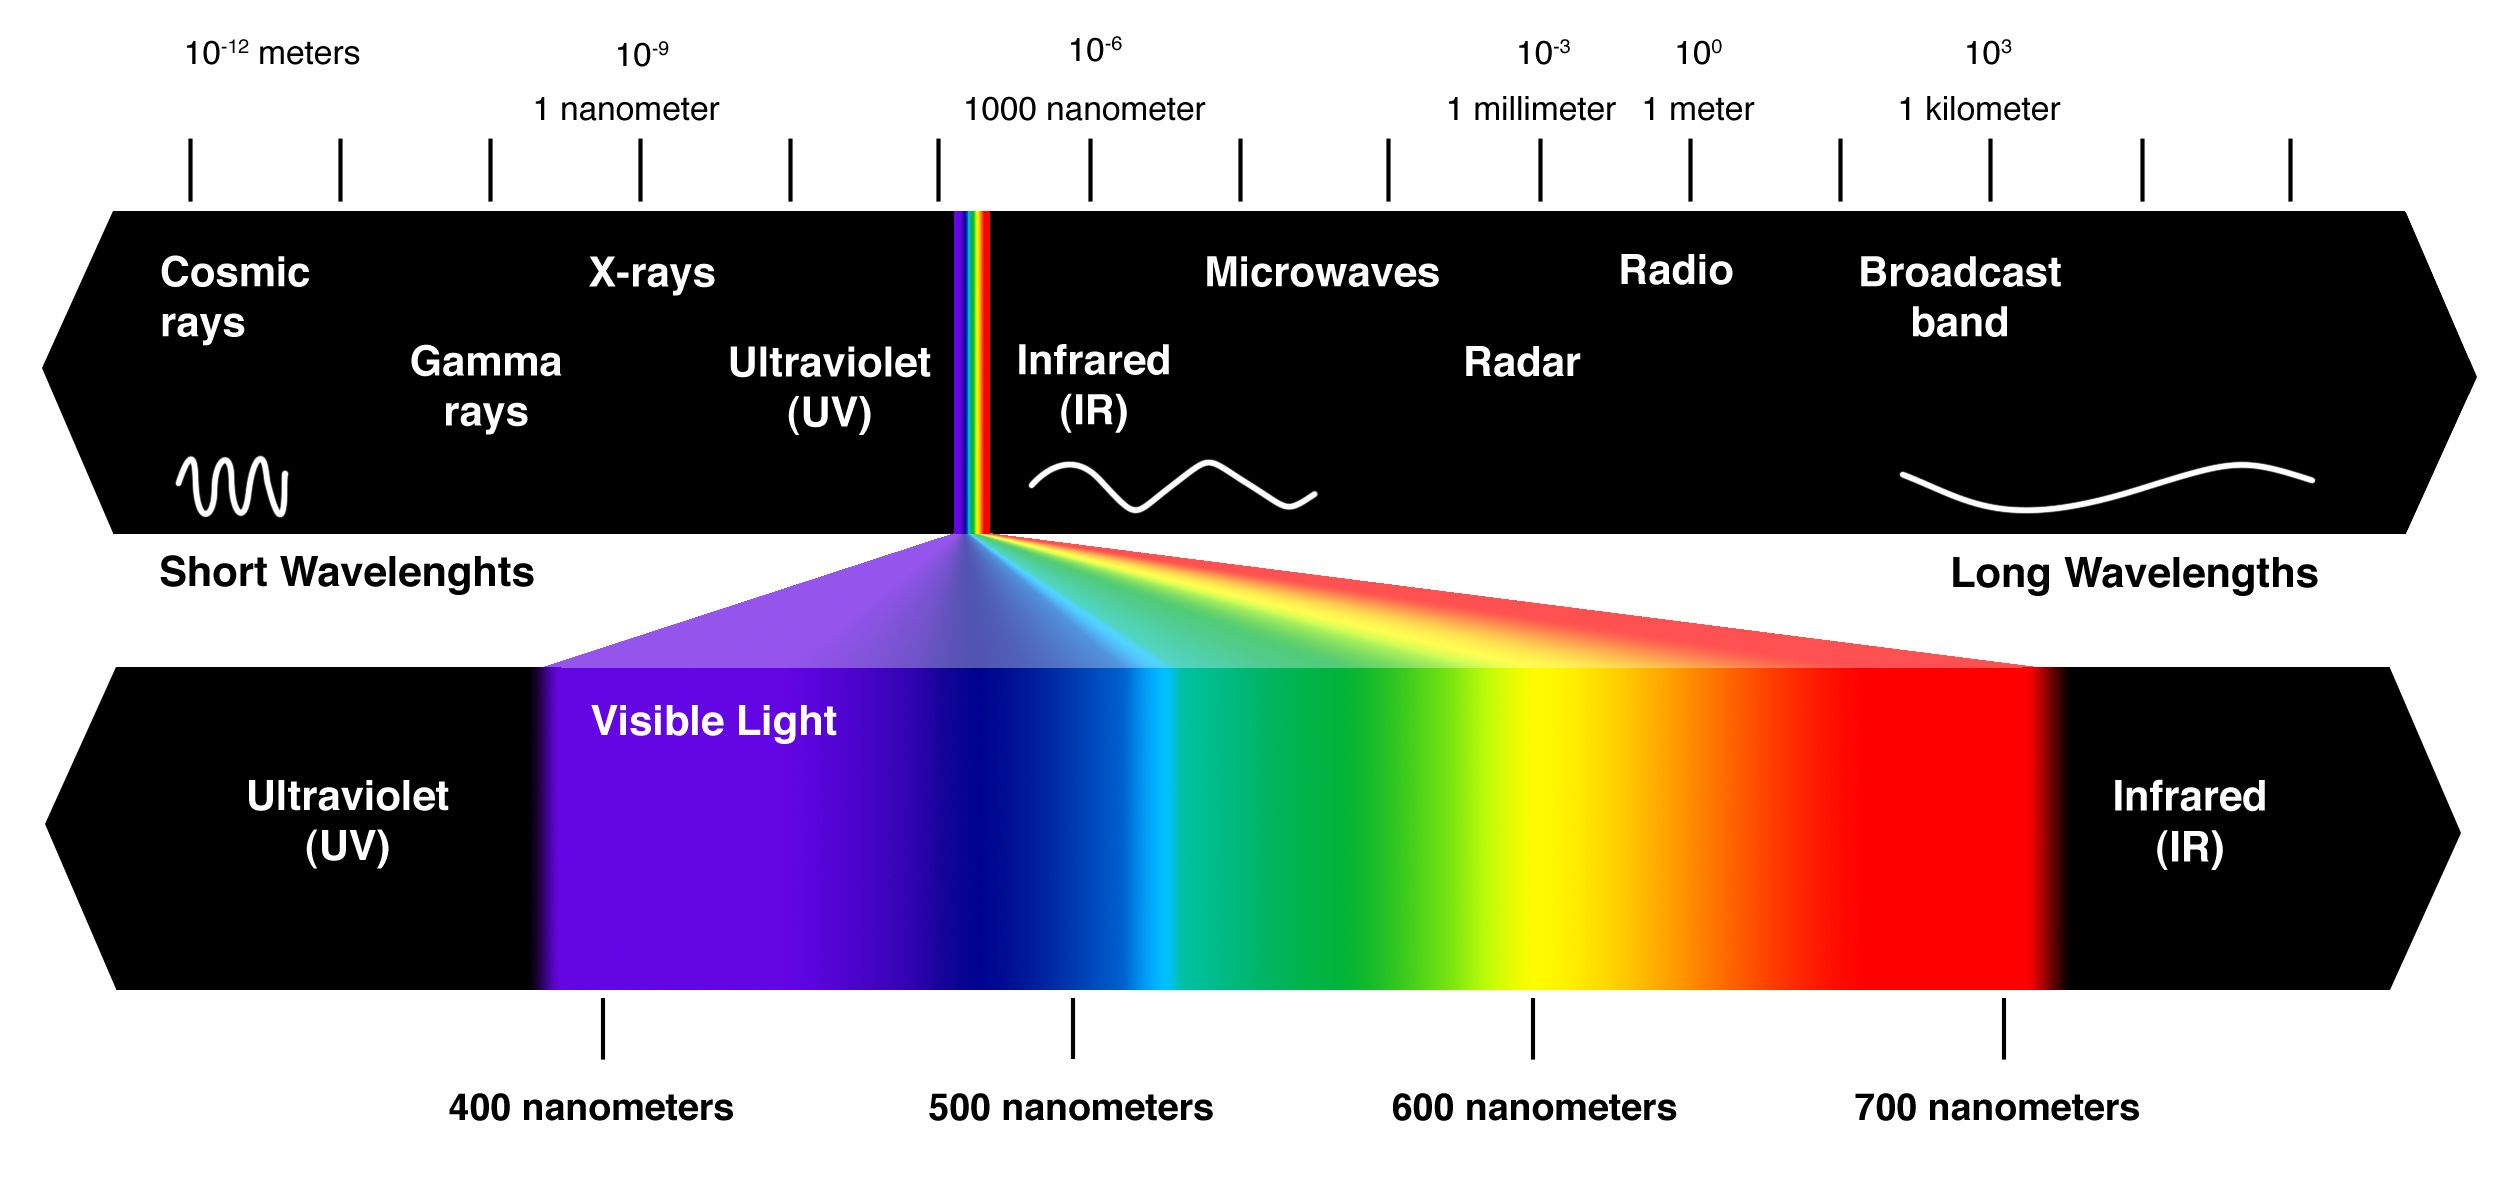
\includegraphics[width=3.5in]{Images/IR Sensor/IR_spectrum.jpg}
	\caption{Infrared Spectrum}
\end{figure}

Based on their range of wave lengths, \ac{IR} can be further classified into three regions. The Near Infrared regions spans from 700nm to 1400nm and is widely used in most of the \ac{IR} sensors and fibre optics. The Mid infrared region spans from 1400nm to 300nm and is mainly used in heat sensing applications. The Far infrared region that spans from 300nm to 1mm is majorly used in thermal imaging. These different region are effectively used to build various application like night vision devices, infrared astronomy, infrared missile tracking etc.

%------------------------------------------------

\section{Types of \ac{IR} sensors}
\par There are various \ac{IR} sensors available in the market. Based on their configuration, we can classify them as Active \ac{IR} sensors and \ac{PIR} sensor . Active \ac{IR} sensors are those sensor capable of both producing and sensing \ac{IR} signals while \ac{PIR} sensors mainly consist of detectors. Most of the motion detectors make use of \ac{PIR}. The \ac{PIR} detects the \ac{IR} signals caused due to the heat energy transmitted by any object. In this chapter we would focus on Active \ac{IR} sensor.

\section{Active \ac{IR} Sensors}
\par An active \ac{IR} sensor consist of both \ac{IR} transmitter and \ac{IR} receiver. The transmitter transmits the \ac{IR} signals which would strike on an object and would bounce back to the receiver. However not all signals are bounced from the surface of the object. The bouncing of signals depends on the colour and material of the object. The dark colors have the ability to absorb more energy and transmit only a small portion of the received light. Light colors on the other hand, reflects most of the received light signals. It is this change of deflection of light that gives us the perception for colors. Since \ac{IR} sensor is only capable of detecting the presence/absence of \ac{IR} signals, they are employed to detect bright/dark surfaces. An \ac{IR} sensor is not capable of differentiating various colors.

\begin{figure}
	\centering
	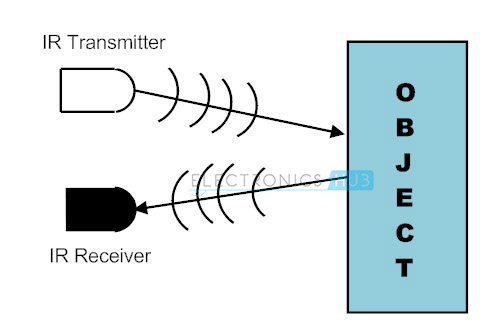
\includegraphics[width=2in]{Images/IR Sensor/IR_wave_bouncing.png}
	\caption{Behaviour of \ac{IR} Sensor}
\end{figure}

\begin{figure}
    \centering
    \subfloat[White surface]{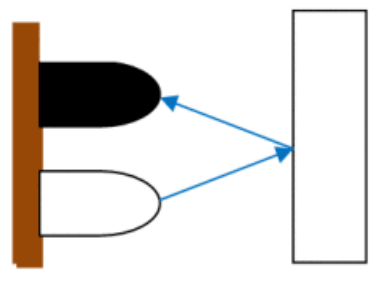
\includegraphics[width=1.5in]{Images/IR Sensor/IR_work_white.png}}\qquad
    \subfloat[Black surface]{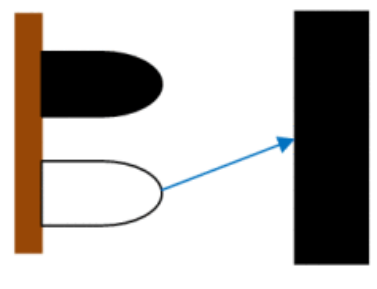
\includegraphics[width=1.5in]{Images/IR Sensor/IR_work_black.png}}
    \caption[]{Working of IR sensor}
\end{figure}

\section{\ac{IR} sensor boards}
Now lets talk about the component required for a complete Active \ac{IR} sensor. An \ac{IR} sensor have two major LED that does the purpose of transmission and detection of signals. A transmission LED looks just like an normal LED diode. Upon applying sufficient voltage across the terminals, the LED produces signals which are transmitted in a straight line. A receiver LED act as an photo-diode that excite electrons upon receiving an \ac{IR} signal. The receiver changes its resistance, which is used to detect the presence of \ac{IR} signal. It is quite easy to identify both the LED. The \ac{IR} receiver would be in dark color to prevent detection of surrounding \ac{IR} signals. Note that the Sun emits a wide range of \ac{EMR}, so it possible for \ac{IR} receiver to detect the \ac{IR} signals from the sunlight. Although it appears just like two LED, we would require proper circuitry to get a calibrated reading. Keep in mind that the receiver and transmitter LED need not always be on the same board, they can have separate circuits to function properly.

\section{Detailing \ac{IR} sensor FC-51}
\par There are various \ac{IR} sensor boards available in the market. You may choose any \ac{IR} sensors suitable for your application. However the underlying principle of \ac{IR} sensor are the same. Here we would make use of \ac{IR} sensor board FC-51 to interface with Arduino.

\begin{figure}
	\centering
	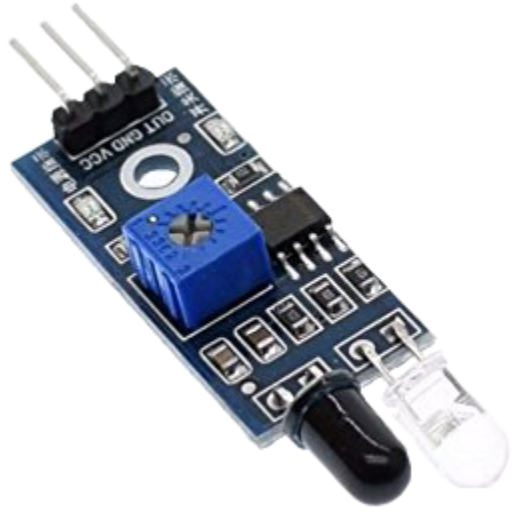
\includegraphics[width=2in]{Images/IR Sensor/IR_board.png}
	\caption{FC-51 IR Sensor board}
\end{figure}

\par A typical \ac{IR} sensor board consist of both the transmitter and receiver diodes along with supporting circuitry which includes a potentiometer, an \ac{IC} and a couple of resistors and LEDs. The potentiometer is used to adjust the sensitivity of the board. The more sensitive the board is, greater will be the amplification of weak signal detected. In other words, it would be able to detect \ac{IR} signal from greater distance. The \ac{IC} would amplify the change in the resistance of \ac{IR} receiver LED and trigger corresponding voltage variations. We can also find two additional indicative LED on the board. One of the LED glows if the board is powered and the other LED glows when the board detects \ac{IR} signals.

\begin{figure}	
	\centering
	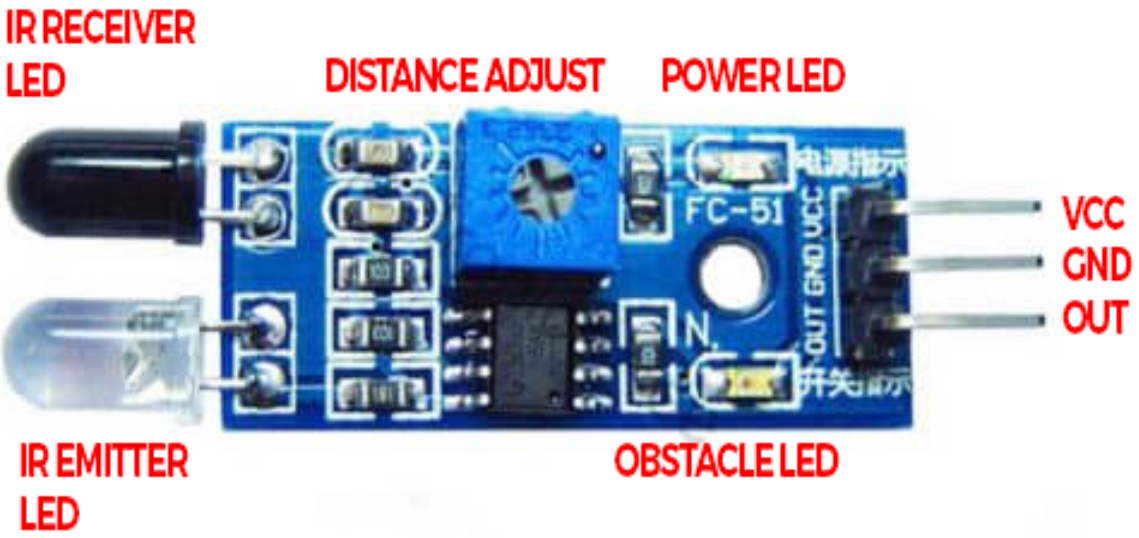
\includegraphics[width=3in]{Images/IR Sensor/IR_board_desp.png}
	\caption{\ac{IR} sensor board description}
	\setfloatalignment{b}
\end{figure}

 Now lets talk about the pins on the board. FC-51 have three legs for interfacing with Arduino. Each legs have there associated marking on the board to indicate what that leg is used for. The VCC pin indicates the power in for the board. The 5v supply from micro-controller is connected to the VCC and the ground (GND) of the board is connected to the GND pin of micro-controller. The OUT pin of the board would act as the input for the Arduino. The OUT pin gives out 5V upon detecting a bright surface and 0V upon detecting a dark surface. There do exist inverted boards that just detects the opposite! ( see table \ref{tab:inverted}) So keep in mind to check board you have before you start coding. 

\begin{table}
    \centering
    \begin{tabular}{|c|c|c|}
    \hline
    \textbf{\hspace{0.4cm}Type of board\hspace{0.4cm}} & \textbf{\hspace{0.4cm} Color of surface\hspace{0.4cm} }& \textbf{\hspace{0.4cm}OUT signal\hspace{0.4cm}} \\
    \hline
    \centering Non inverted & Bright & 5V(high) \\ \cline{2-3} & Dark & 0V(low) \\
    \hline
    \centering Inverted & Bright & 0V(low) \\ \cline{2-3} & Dark & 5V(high) \\
    \hline
    \end{tabular}
    \caption{Inverted and Non-inverted IR boards}
    \label{tab:inverted}
\end{table}

\hspace{0.5cm}
\par Usually in an digital circuit, voltage below 2.3v is regarded as a low signal ( 0v | binary zero) and those above 2.5v as high signal ( 5v | binary 1). There do exist \ac{IR} sensor boards that provide analog output reading. Make sure to understand the configuration of the board before interfacing with Arduino. With that, let start coding. Since FC-51 gives digital output ( HIGH | LOW ) we would be using digital pin of Arduino to interface.

\section{\textbf{Code example 1}}
Objective: Program to print the status of \ac{IR} sensor to Serial monitor

\begin{lstlisting}[style=CStyle]
int IR_pin = 2;    //connect OUT pin of IR to 2nd pin of Arduino

void setup(){

    pinMode(IR_pin,INPUT);    //IR as an input signal
    Serial.begin(9600);       //Baud rate
}

void loop(){
    
    //Reading the digital state of IR_pin
    int state = digitalRead(IR_pin);	
    
    if( state == HIGH){
        Serial.println("Bright surface detected");
    }
    else{
        Serial.println("Dark surface detected");
    }
    
    //Slow down the code so that serial monitor
    // does not flood with characters
    delay(500);
} 
\end{lstlisting}

\begin{figure}	
	\centering
	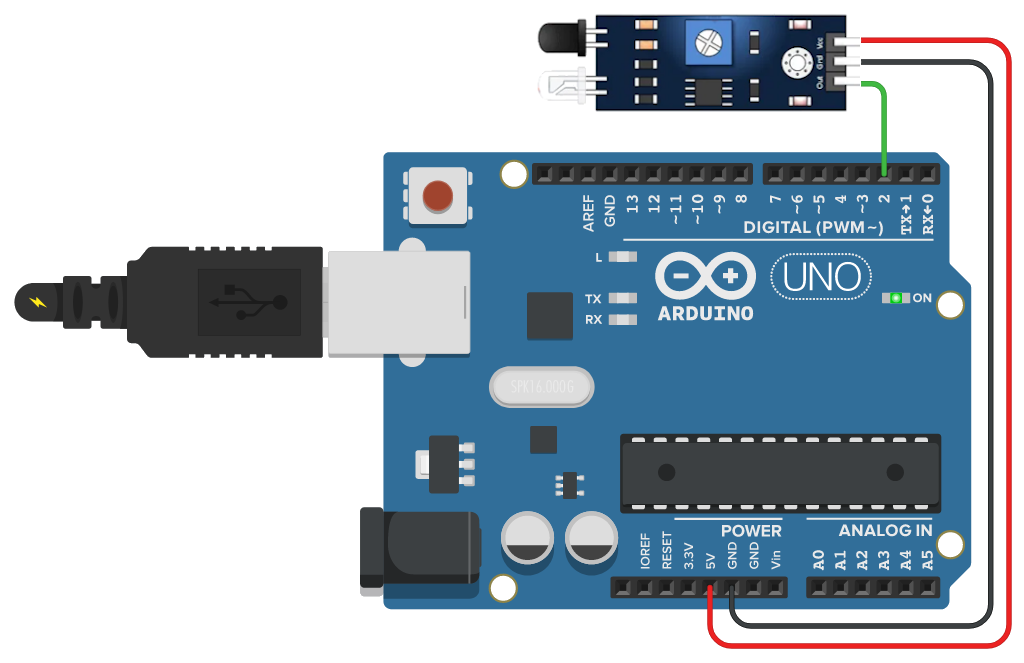
\includegraphics[width=4in]{Images/IR Sensor/circuit1.png}
	\caption{Interfacing \ac{IR} with Arduino}
	\setfloatalignment{b}
\end{figure}

\par Set the serial monitor at 9600 baud rate and see the results. We can find that when there is no object in front of sensor or in the presence of a dark object, the serial monitor shows "Dark surface detected". The monitor would show "Bright surface detected" when there is a white/reflective surface is introduced. Keep in mind that the sun light/flames also emit \ac{IR} radiations that can be detected by \ac{IR} sensors.

\section{\textbf{Code example 2}}
Objective: Program to turn on the in-build LED at pin 13 of Arduino Uno if \ac{IR} sensor detects a while surface. Else keeps the LED off. The circuit of previous example can be used.

\begin{lstlisting}[style=CStyle]
int IR_pin = 2;
int LED = 13;

void setup(){
    pinMode(IR_pin,INPUT);
    pinMode(LED,OUTPUT);
}
void loop(){
    int state = digitalRead(IR_pin);
    digitalWrite(LED, state);
    
    //alternatively use the single line code
    //digitalWrite(LED,digitalRead(IR_pin));
    
    delay(200);
}
\end{lstlisting}


\section{Line Follower bot}

\par Line follower bot is an simple bot that make use of \ac{IR} sensors. The bot consist of \ac{IR} sensors ( usually an \ac{IR} sensor array - figure \ref{fig:ir_array}), wheel and motors, motor driver, Voltage source all placed in a chassis. An \ac{IR} array is a collection of 4 to 6 \ac{IR} sensor receive and transmitter. We would be reading values from individual pair of sensors. Another major component is the motor driver. As the name suggests, they are used to drive motors. Jump to the chapter \ref{chap:Motor_Driver} to setup the bot - wheels and motors.

\begin{marginfigure}	
	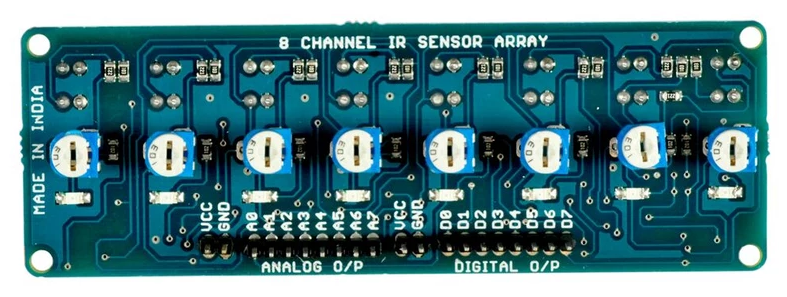
\includegraphics{Images/IR Sensor/IR_array.png}
	\caption{\ac{IR} Array}
	\label{fig:ir_array}
\end{marginfigure}

Line follower bot follows a line to its destination. To detect the more precisely, the paths is formed by black lines in a white background or white path in black background. Usually the later is chosen as it is easy to construct black path in white background. For this simple bot, we would be making use of two \ac{IR} sensors instead of an \ac{IR} array. Our bot would have two wheels instead of four, although it is easy to extend to four wheels.

\begin{figure}
    \subfloat[\ac{IR} Bot]{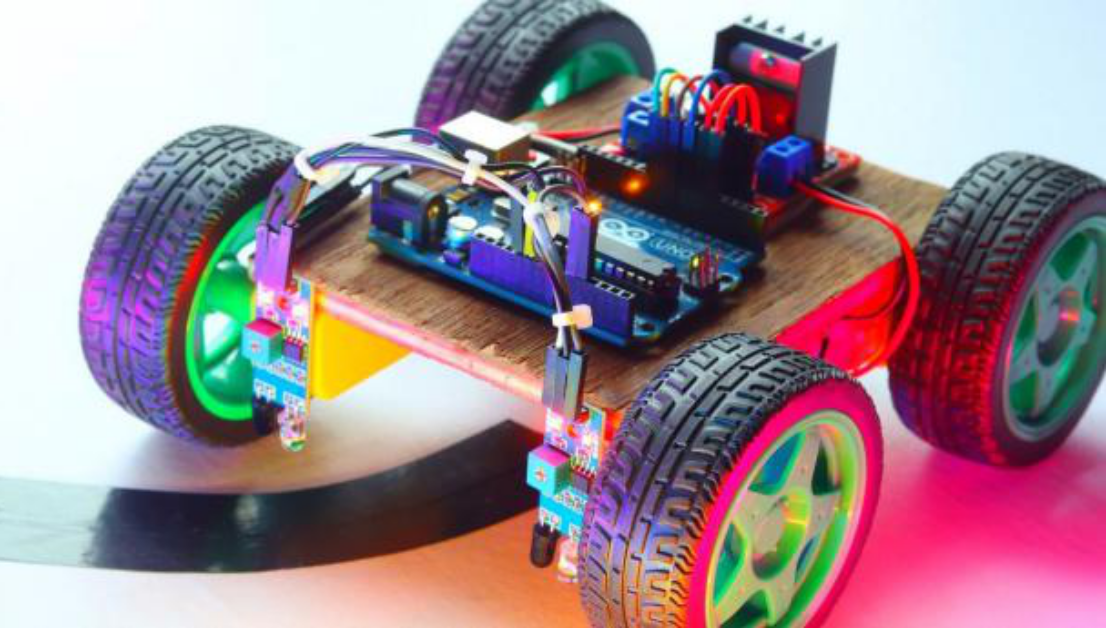
\includegraphics[width=2in]{Images/IR Sensor/line_follower_bot1.png}}
    \quad
    \subfloat[Line follower path]{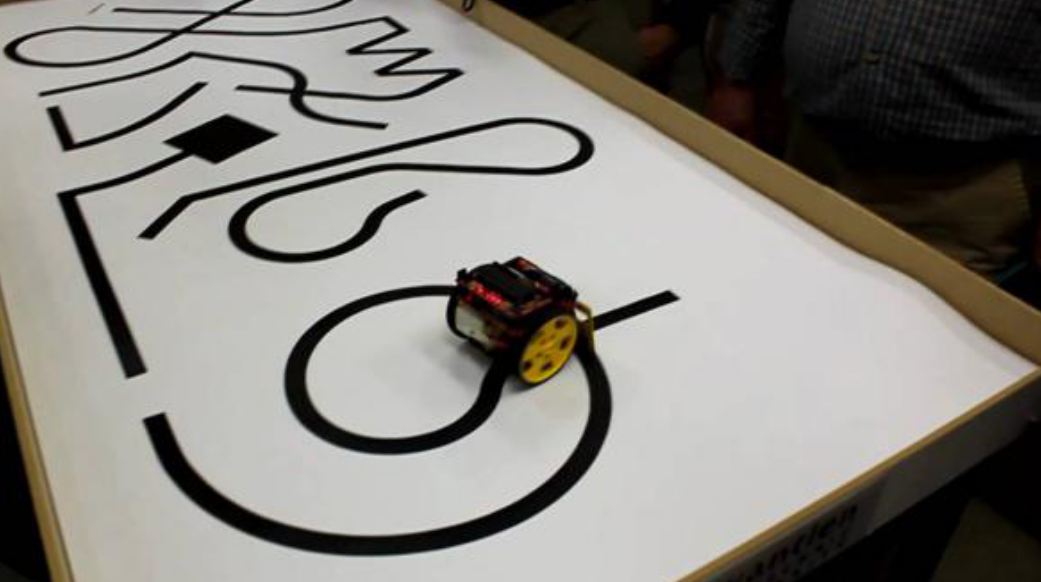
\includegraphics[width=2in]{Images/IR Sensor/line_follower_path.png}}
    \caption{Line follower - bot and path}
\end{figure}

\section{Tracing line - Line follower}

The main event of the line follower is to trace the line. In our sample environment, we would be using two \ac{IR} sensors to detect the black line on the while surface. The bot is placed such that the black line moves right through the center of the bot. Both the sensors are places right next to the dark line.

\begin{marginfigure}
    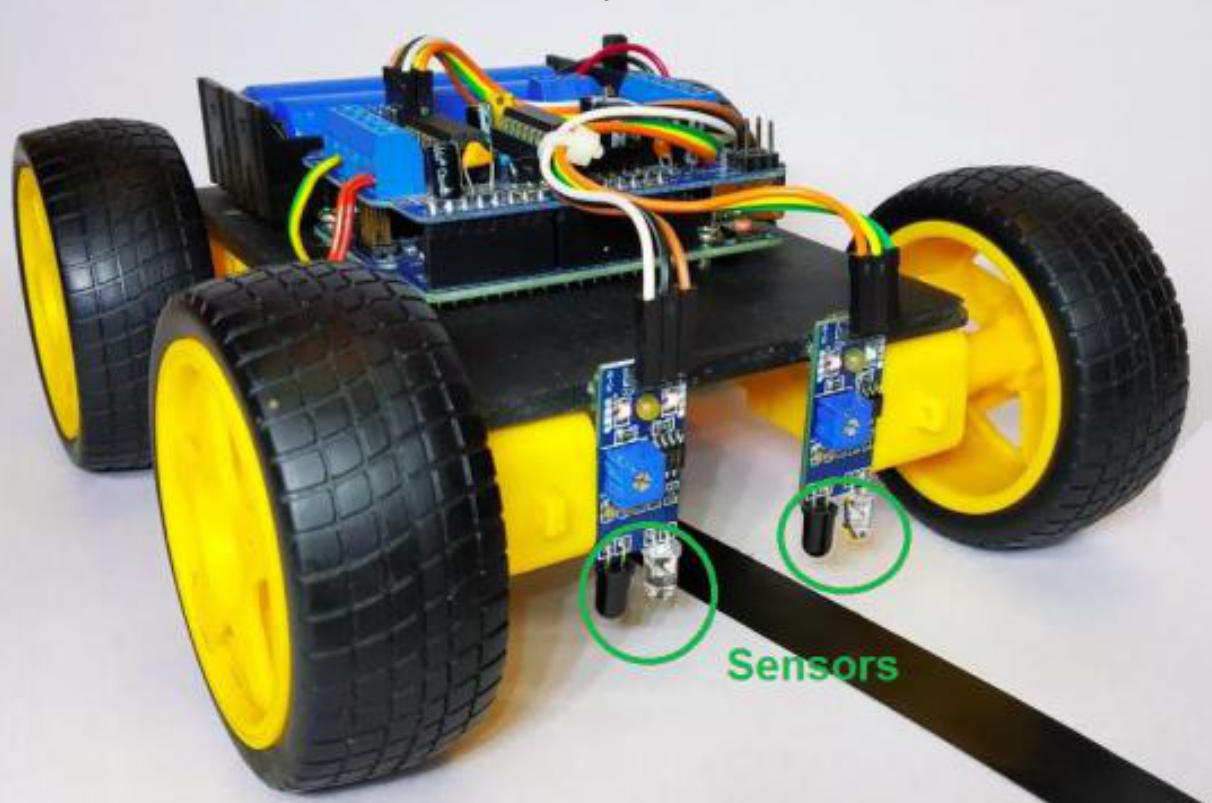
\includegraphics{Images/IR Sensor/sensor_align.png}
     \caption[Line Follower Sensor]{Line follower sensor alignment}
\end{marginfigure}

Table \ref{tab:line_follower_move} have listed all sort of possible combinations with 2 \ac{IR} sensors. Now lets implement them in our bot. Take a quick peek at the section \ref{section:bot_interface} where we have programmed a small bot. Lets add the additional \ac{IR} sensors to them to complete our line follower.

\renewcommand{\arraystretch}{3.6}
\begin{table}
    \centering
    \begin{tabular}{|c|c|c|c|c|}
    \hline
        \textbf{Path property} & \textbf{Left IR} & \textbf{Right IR} & \textbf{Reaction of the bot} & \textbf{Scenario} \\ \hline
        Straight path & HIGH (white) & HIGH (white) & Forward motion & \begin{minipage}{.3\textwidth}
            \centering
            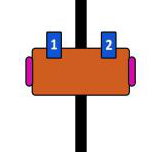
\includegraphics[width=\linewidth, height=20mm]{Images/IR Sensor/IR_linefollower_straight.png}
            \vspace{1mm}
        \end{minipage} \\ \hline
        Makes a right curve & HIGH (white) & LOW (black) & Turn right & \begin{minipage}{.3\textwidth}
            \centering
            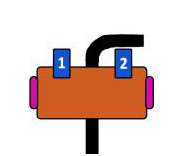
\includegraphics[width=\linewidth, height=20mm]{Images/IR Sensor/IR_linefollower_right.png}
            \vspace{1mm}
        \end{minipage}  \\ \hline
        Makes a left curve & LOW (black) & HIGH (white) & Turn left & \begin{minipage}{.3\textwidth}
            \centering
            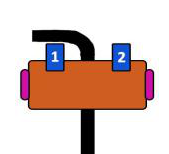
\includegraphics[width=\linewidth, height=20mm]{Images/IR Sensor/IR_linefollower_left.png}
            \vspace{1mm}
        \end{minipage}  \\ \hline
        Cross bar & LOW (black) & LOW (black) & Stop & \begin{minipage}{.3\textwidth}
            \centering
            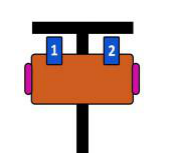
\includegraphics[width=\linewidth, height=20mm]{Images/IR Sensor/IR_linefollower_stop.png}
            \vspace{1mm}
        \end{minipage}  \\ \hline
    \end{tabular}
    \setfloatalignment{b}
    \vspace{9mm}
    \caption{Line follower movement}
    \label{tab:line_follower_move}
\end{table}
\renewcommand{\arraystretch}{1}

\begin{figure}
    \centering
    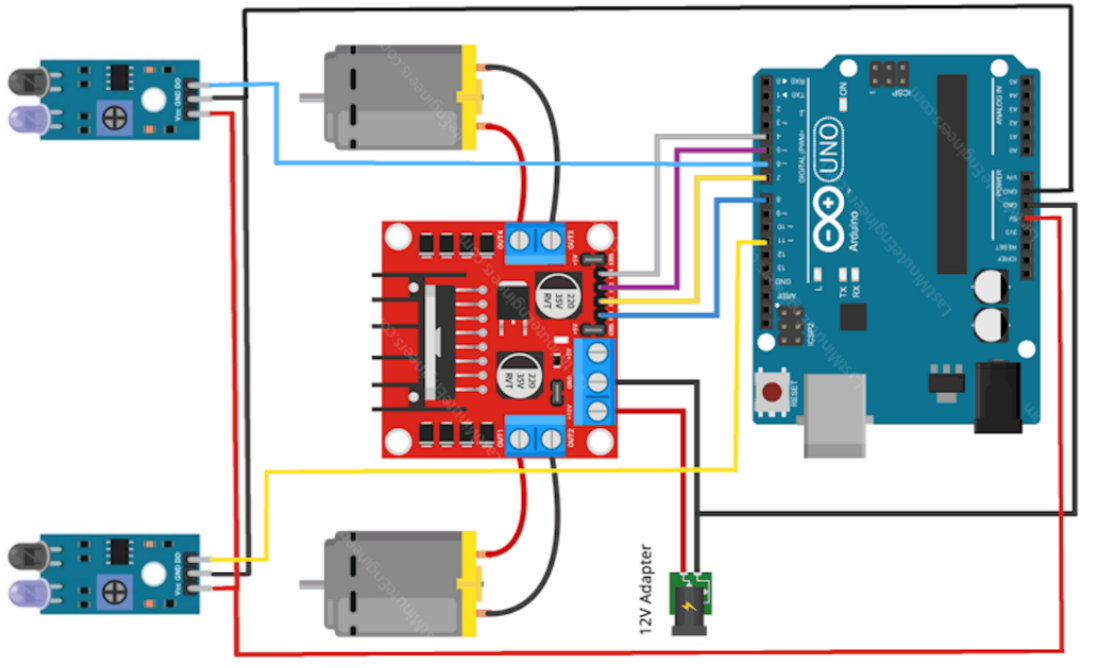
\includegraphics{Images/IR Sensor/ir_bot.png}
     \caption{\ac{IR} Line follower Circuit}
     \label{fig:ir_bot}
\end{figure}

\par Lets detail the connection of the circuit show in figure \ref{fig:ir_bot}. The VCC and GND of \ac{IR} sensors are connected to 5V and GND of Arduino. The left \ac{IR} sensor (bottom) gives its output to 11th pin of Arduino while the right \ac{IR} sensor (top) gives its output to 6th pin of Arduino. The GND of motor driver is connected to the GND of Arduino and input1, input2, input3, input4 of driver are connected to pins 8, 7, 5, 4 pins of Arduino respectively. Left motor is connected to the channel A and right motor is connected to channel B of the motor driver. Finally we powered the driver using a 12v adapter and connected the GND of driver and Arduino to it. Now lets implement the logic depicted on the table \ref{tab:line_follower_move}.

\begin{lstlisting}[style=CStyle]
int m1 = 8, m2 = 7;    //left  motor pins
int m3 = 5, m4 = 4;    //right motor pins
int ir1 = 11, ir2 = 6; //left and right \ac{IR} sensor inputs

void setup(){
    //set motor pins as output for Arduino.
    pinMode(m1,OUTPUT); pinMode(m2,OUTPUT);
    pinMode(m3,OUTPUT); pinMode(m4,OUTPUT);
    
    //set IR pins as input for Arduino
    pinMode(ir1, INPUT); pinMode(ir2, INPUT);
    
    Serial.begin(9600);
}

//A function to control motor movement
void turn_motor(int input1, int input2, char dir){
    if( dir == 'F'){
        //clockwise rotation
        digitalWrite(input1,HIGH);
        digitalWrite(input2,LOW);
    }
    else if( dir == 'S'){
        //no rotation
        digitalWrite(input1,LOW);
        digitalWrite(input2,LOW);
    }
}

void loop(){
    //reading the IR sensors
    int left  = digitalRead(ir1);
    int right = digitalRead(ir2);
    
    if( left == HIGH && right == HIGH){//Forward motion
        turn_motor(m1, m2, 'F');           
        turn_motor(m3, m4, 'F');           
        Serial.println("Bot moving forward");
    }
    else if(left == HIGH && right == LOW){//Right motion
        turn_motor(m1, m2, 'F'); 
        turn_motor(m3, m4, 'S');
        Serial.println("Bot turning right");
    }
    else if(left == LOW && right == HIGH){//Left motion
        turn_motor(m1, m2, 'S');  
        turn_motor(m3, m4, 'F'); 
        Serial.println("Bot turning left");
    }
    else{								//Stopping the bot
        turn_motor(m1, m2, 'S');
        turn_motor(m3, m4, 'S');
        Serial.println("Bot paused");
    }
    delay(100);
}
\end{lstlisting}

\par You might have noticed that the bot drifts or becomes unstable when it changes it direction suddenly. This is because the wheels are rotating with higher speed than our bot can handle. The solution to such problems is the control the speed of the wheels. Refer the section \ref{section:speed_controlled_bot} to build speed controlled bot. You may also find that bot travels in a zig-zag fashion, the curves are not covered smoothly or the bot may miss some sharp curves. To avoid such problems, line followers are build using an \ac{IR} array, where there are more sensors to detect the intensity of curves etc. 

\paragraph{ } Line follower is one of the popular projects in Arduino-ROBOTICS. Various competitions are held across the world with varying difficulty and challenges. Maze solver is one of the most common event held. Speed, accuracy and reliability of bots are noted to announce the winner. To improve the probability of bagging the price, various statistical theories, mathematical models are applied and coded into the programs. Here we have detailed the basics of line follower. The rest is left to you to explore!

\begin{figure}
    \centering
    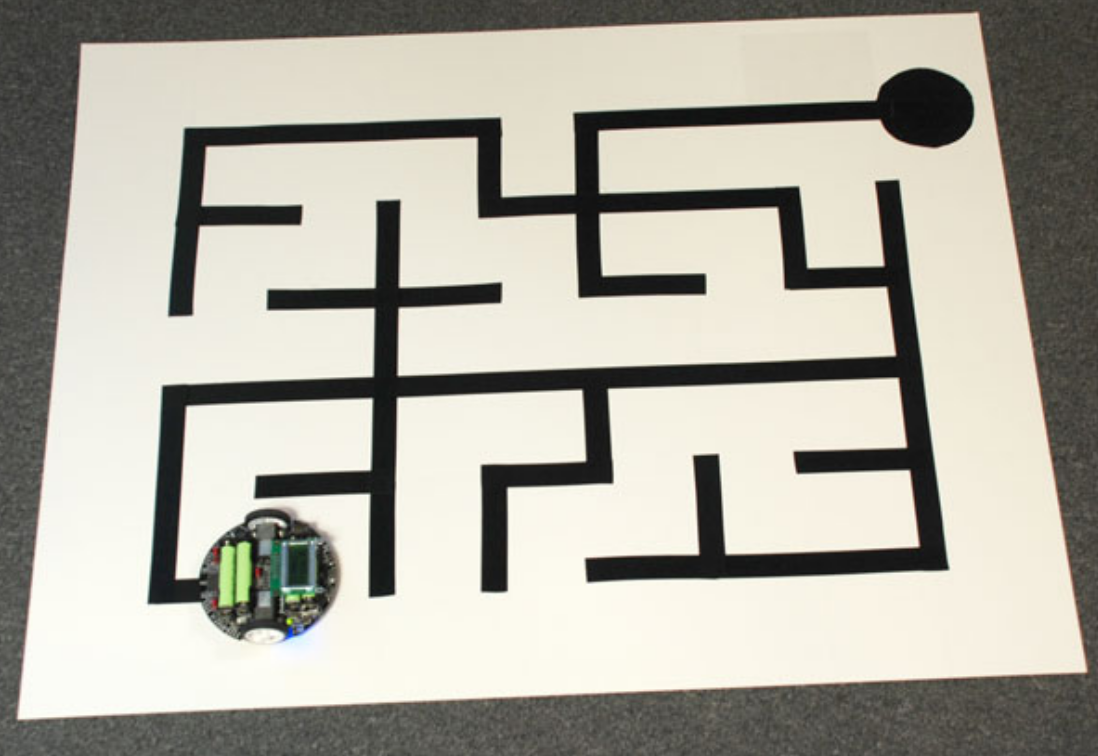
\includegraphics{Images/IR Sensor/line_maze.png}
    \caption{Line follower maze}
\end{figure}

%----------------------------------------------------------------------------------------
%	CHAPTER 6 : Interfacing UltraSonic sensors
%----------------------------------------------------------------------------------------
\chapter{Interfacing UltraSonic sensors}
\label{ch:ultrasonic}
%------------------------------------------------

\justify
 \section{What is meant by ultra-sonic waves ?}
Defined by the American National Standards Institute, a ultra-sound are sound frequencies greater than 20Khz. They are normal sound waves which humans cannot hear, but some animals can. Humans ears can detect sound of frequencies in the range from 20Hz to 20KHz. Ultra sonic waves behave similar to normal sound waves i.e., they propagate at 340m/s and reflects upon striking a surface. They are widely employed in detection and raging, imaging, under water communication etc.
\hspace{2cm}
\begin{figure}[h!]	
	\centering
	\includegraphics[width=3in]{Chapters/images/ultraSonic_spectrum.png}
	\caption{The Ultrasonic Spectrum}
	\setfloatalignment{b}
\end{figure}

 The production of ultrasonic waves requires a transmitter that transmit wave pulses, which are then received by a receiver. These two unites are imprinted in a board to be synchronous in achieving the task. The sensor is controlled by digital signals (pulses), produced/controlled by micro controllers or processors. 
%------------------------------------------------

\section{Ultrasonic sensor}
There are various series of ultrasonic sensor available. They differ in their functionality on the projects. Few sensors have higher sensitivity, other few have more or less number of connection pins etc. The utility of each sensor is based on the projects they are used. Few sensors can be preferred more that other sensor in a particular project. In this session, we would be detailing about HC-SR04,  one of the commonly used ultrasonic sensors.
\begin{figure}
    \centering
    \includegraphics[width=3in]{Chapters/images/ultraSonic_board.png}
    \caption{Ultrasonic Sensor}
	\setfloatalignment{b}
\end{figure}

\section{Detailing HC-SR04 ultrasonic sensor}
HC-SR04 is the most commonly used ultrasonic sensor. It is interfaced with Arduino via four pins. The board have a two cylinder like structures with a mesh/net on them. They are the transmitter and receivers made up of crystals of materials such as quartz that vibrate very fast when electricity is passed through them—an effect called “piezoelectricity.” As they vibrate, they manipulate the air around them and the fluids they come in contact with, producing ultrasonic waves. In transmitter the electricity is passed to the crystal to produce waves. In the receiver, the vibrating crystal produce small voltages that are detected and amplified. The cylinder that transmit waves have a small marking “T” at the edge and the receiver have a “R” marking at its edge. To synchronize the activity, the board has and 4Mhz oscillator to act as a timer. This specific board can detect an object if it is between 2-40cm range in front of the sensors.\\
\vspace{1cm}
\hspace{2cm}
\begin{figure}[h!]	
	\centering
	\includegraphics[width=4in]{Chapters/images/ultraSonic_desp.png}
	\caption{Ultrasonic Sensor Board Description}
	\setfloatalignment{b}
\end{figure}
\hspace{2cm}
\section{Pins on HC-SR04}
The board have 4 pins, they are VCC, TRIG, ECHO, GND. To power up the sensor, 5V and GND of Arduino are connected to the VCC and GND pins of the sensor. The TRIG is the input pin, that denote how long should the sensor produce ultrasonic waves. The ECHO is the output pin that denotes how long have we waited to receive the ultrasonic wave. Keep in mind that the input of the sensor will be connected to the output pin of Arduino and the output pin of sensor will be interfaced as input pin for Arduino. In short, the signal travels from sensor to Arduino in ECHO pin and from Arduino to sensor in TRIG pin.
\\

\section{Working of HC-SR04 sensor}

\begin{figure}[hbt!]	
\begin{multicols}{2}{}{}
	\includegraphics[width=1.6in]{Chapters/images/ultraSonic_working_trans.png}\hspace{0.6cm}
	\includegraphics[width=1.6in]{Chapters/images/ultraSonic_working_recv.png}
	\caption{Ultrasonic Sensor Working}
	\setfloatalignment{b}
\end{multicols}
\end{figure}
Initially we would put TRIG pin high for about 10 micro seconds. The sensor, upon receiving this signal, produce eight 40KHz pulses automatically. After producing short pulse burst, it would start the timer and pulls the ECHO pins to a high signal. It would then wait for the transmitted signal to reach back to the sensor. Upon receiving the first wave, it pulls the ECHO pin to low. We would record the time the ECHO pin remained high to calculate the distance between the sensor and the object.
\\
\section{Calculation of the distance}
We know that 
\begin{align*}
    speed &= \frac{distance}{time}
\end{align*}
Or,
\begin{align*}
    distance &= speed * time
\end{align*}  
\\ We have 
    speed of sound = 340m/s
\\Time can be fetched from the ultrasonic sensors.
\\Do note that the speed is in m/s and the time we receive is in µs. Lets formulate a formula to convert the units so that the distance can be measured in centi-meters (cm).
\\Let ‘ t ’ denote the time we get from sensor in µs. Keep in mind that this time it the time taken by the waves to travel from sensors to the object and back to the sensors. In short, they have covered the distance twice. So the time required by the wave to travel from sensors to object is t/2 µs. Lets substitute the values in the formula
\begin{align*}
    distance &= 340 m/s * \frac{t}{2} \hspace{0.1cm} \mu s \\
    distance &= 340 * \frac{t}{2} \hspace{0.1cm} \frac{m \mu s}{s} \\
    distance &= 170t\hspace{0.1cm} \mu m \\
    distance &= 170t * 10^{-6} \hspace{0.1cm} m \\
    distance &= 170t * 10^{-4} \hspace{0.1cm} cm \\
    \vspace{0.3cm} \\
    distance &= 0.017t \hspace{0.1cm} cm \\
\end{align*}


\section{\textbf{Code example 1}}
Objective : To print the distance of a object from sensor in serial monitor. \\
\vspace{0.2cm}
\begin{lstlisting}[style=CStyle]

int TRIG = 10;					//trigger pin of sensor
int ECHO = 9;					//echo pin of sensor
long duration;					//to store the time micro seconds
float distance;					//to store the distance cm

void setup(){
pinMode(TRIG,OUTPUT);		//TRIG as output of Arduino
pinMode(ECHO,INPUT);			//ECHO as input of Arduino
Serial.begin(9600);			//Baud rate that serial monitor listens to
}

void loop(){
//wait for some time to clear the ultrasonic waves if present in environment
digitalWrite(TRIG,LOW);
delayMicroseconds(2);

//create ultrasonic burst
digitalWrite(TRIG,HIGH);
delayMicroseconds(10);
degitalWrite(TRIG,LOW);

//record the duration ECHO pin stood HIGH
duration = pulseIn(ECHO,HIGH);

//calculate the distance
distance = 0.017 * duration;

//print the distance
Serial.print("The object is at ");
Serial.print(distance);
Serial.println(" cm");

delay(1000);					//Slow down the code so that serial monitor
// does not flood with characters
}
\end{lstlisting}
\vspace{0.5cm
}
\begin{figure}[h!]	
	\centering
	\includegraphics[width=4in]{Chapters/images/ultraSonic_circuit1.png}
    \caption{Interfacing Ultrasonic Sensor with Arduino}
	\setfloatalignment{b}
\end{figure}
\vspace{0.5cm}

It is always advised to to wait for at least 2µs to clear the already existing ultrasonic wave in the environment. Try moving the hand in front of sensor to see varying distances. What would happen if we kept our hand on the sensor ( i.e. 0cm distance)? Why does it show high value instead of printing zero? Keep in mind that the receiver need to detect some ultrasonic waves to pull the ECHO pin down.

\section{Object avoider-bot}
Let us now try to create a bot that can avoid the objects in front of it and keep travelling. There are various models of such bot available. In this session we would be making use of two ultrasonic sensors and a bot (with chassis, motor, motor driver, wheel) to construct an object avoider bot. Get an peek into the chapter “Motor Driver” to know various part of constructing a bot. We would be making use of bot build in the chapter “Motor Driver” to construct our object avoider bot.
\vspace{0.5cm}
\begin{figure}
    \centering
    \includegraphics[width=3in]{Chapters/images/ultraSonic_bot.png}
    \caption{Obstacle Avoider Bot}
	\setfloatalignment{b}
\end{figure}


We will be programming the bot to avoid the obstacle if it comes less than 10cm in front of the bot. The following table summarizes our flow.

\begin{table}[h!]
    \begin{tabular}{|c|c|c|c|}
    \hline
    \textbf{Left Ultrasonic Sensor}& \textbf{Right Ultrasonic sensor} & 
    \textbf{Reaction of the bot} &
    \textbf{Scenario} \\
    \hline
    >10cm & >10cm & Forward motion &
    \parbox[c]{6em}{ \includegraphics[width=0.7\textwidth,height=20mm]{Chapters/images/ultraSonic_objAvoider_straight.png}} \TBstrut \\
    \hline
    >10cm & <=10cm & Turn left &
    \parbox[c]{6em}{    \includegraphics[width=0.7\textwidth,height=20mm]{Chapters/images/ultraSonic_objAvoider_left.png.png}} \TBstrut \\
    \hline
    <=10cm & >10cm & Turn right &
    \parbox[c]{6em}{    \includegraphics[width=0.7\textwidth,height=20mm]{Chapters/images/ultraSonic_objAvoider_right.png}} \TBstrut \\
    \hline
    <=10cm & <=10cm & Default: Rotate left &
    \parbox[c]{6em}{    \includegraphics[width=0.7\textwidth,height=20mm]{Chapters/images/ultraSonic_objAvoider_rotate.png}} \TBstrut \\
    \hline
    \end{tabular}
\end{table}
\vspace{2cm}
Here we have listed all sort of possible combinations with 2 IR sensors. Now lets implement them in our bot. Take a quick peek at the chapter "Motor Driver" where we have programmed a small bot. Lets add the addition IR sensors to them to complete our line follower.

\begin{figure}
    \centering
    \includegraphics{Chapters/images/ultraSonic_objAvoider_circuit.png}
     \caption{Obstacle Avoider Circuit}
	\setfloatalignment{b}
\end{figure}
\vspace{1cm}
Lets simplify the connections. First connect motors to motor driver. Now lets interface motor driver with Arduino Uno. Connect the pins input1, input2, input3, input4 of motor drive to Arduino pins 8, 7, 5 and 4 receptively. The left ultrasonic sensor (top) have its TRIG and ECHO pins connected to 12 and 11 pins of Arduino. Connect its VCC and GND to Arduino 5V and GND respectively. The right ultrasonic sensor (bottom) have its TRIG and ECHO pins connected to 3 and 2 pins of Arduino. Connect its VCC to 5V pin of motor driver and GND to GND pin of Arduino. Each ultrasonic sensor needs separate 5V line. If there are no other 5V source, then you can set any unused pin of Arduino to HIGH and extract 5V from that pin. Finally connect the 12V power line to 12V pin of motor driver and GND pin of motor driver to GND of Arduino and the negative terminal of the 12V source. Power the Arduino using USB cable. With that we have completed the circuits. Now lets build the code.

\vspace{0.5cm}
Code :
\begin{lstlisting}[style=CStyle]
int m1 = 8, m2 = 7;  			//left  motor pins
int m3 = 5, m4 = 4;  			//right motor pins
int trig_L = 12, echo_L = 11; 	//left ultrasonic sensors
int trig_R = 3, echo_R = 2; 		//right ultrasonic sensors
float distance_L, distance_R;		//to store each distances
long duration;					//to store time temporarily
float obj_dist = 10.0;			//threshold distance

void setup(){
//set motor pins as output for Arduino.
pinMode(m1,OUTPUT); pinMode(m2,OUTPUT);
pinMode(m3,OUTPUT); pinMode(m4,OUTPUT);

//set TRIG pins as OUTPUT and ECHO pins as INPUT
pinMode(trig_L,OUTPUT); pinMode(echo_L,INPUT);
pinMode(trig_R,OUTPUT); pinMode(echo_R, INPUT);

Serial.begin(9600);
}

//A function to control motor movement
void turn_motor(int input1, int input2, char dir){
if( dir == 'F'){
//clockwise rotation
digitalWrite(input1,HIGH);
digitalWrite(input2,LOW);
}
else if( dir == 'B'){
//anti-clockwise rotation
digitalWrite(input1,LOW);
digitalWrite(input2,HIGH);
}
else if( dir == 'S'){
//no rotation
digitalWrite(input1,LOW);
digitalWrite(input2,LOW);
}
}

void loop(){

// reading value from left sensors
digitalWrite(trig_L,LOW);
delayMicroseconds(2);
digitalWrite(trig_L,HIGH);
delayMicroseconds(10);
degitalWrite(trig_L,LOW);
duration = pulseIn(echo_L,HIGH);
distance_L = 0.017 * duration;

// reading value from right sensors
digitalWrite(trig_R,LOW);
delayMicroseconds(2);
digitalWrite(trig_R,HIGH);
delayMicroseconds(10);
degitalWrite(trig_R,LOW);
duration = pulseIn(echo_R,HIGH);
distance_R = 0.017 * duration;

if( distance_L > obj_dist && distance_R > obj_dist ){			//forward
turn_motor(m1, m2, 'F');  //left  wheel : clockwise
turn_motor(m3, m4, 'F');  //right wheel : clockwise
Serial.println("Bot moving forward");
}
else if( distance_L > obj_dist && distance_R <= obj_dist ){		//left
turn_motor(m1, m2, 'S');  //left  wheel : stop
turn_motor(m3, m4, 'F');  //right wheel : clockwise
Serial.println("Bot moving left");
}
else if( distance_L <= obj_dist && distance_R > obj_dist ){		//right
turn_motor(m1, m2, 'F');  //left  wheel : clockwise
turn_motor(m3, m4, 'S');  //right wheel : stop
Serial.println("Bot moving right");
}
else if( distance_L <= obj_dist && distance_R <= obj_dist ){	//rotate left
turn_motor(m1, m2, 'B');  //left  wheel : anti-clockwise
turn_motor(m3, m4, 'F');  //right wheel : clockwise
Serial.println("Bot rotating left");
delay(1000); 	//let the bot rotate a bit!!
}
delay(100);
}

\end{lstlisting}
\vspace{1cm}
Try out the same bot by controlling the speeds of wheels. Setup a dummy cardboard maze puzzle and try to solve the puzzle using the bot. You might need to make use of additional concepts to effectively navigates through the edges of walls. You could also rebuild the object avoider bot using single ultrasonic sensor and a servo motor. Put your thoughts and imaginations to get new ideas and solve new challenges.
\vspace{0.5cm}
\begin{figure}
\begin{multicols}{2}
    \centering
    \includegraphics[width=2.2in]{Chapters/images/ultraSonic_objAvoider_path.png}
    \includegraphics[width=2.3in]{Chapters/images/ultraSonic_end_pic.png}
    \caption{Obstacle Avoider Bots}
	\setfloatalignment{b}
\end{multicols}
\end{figure}

%----------------------------------------------------------------------------------------
%	CHAPTER 7 : Interfacing DTMF
%----------------------------------------------------------------------------------------
\chapter{Interfacing DTMF}
\label{ch:dtmf}
%------------------------------------------------

\ac{DTMF} is a common method used by phone companies to conduct surveys and other requests. It is a telecommunication signaling system using the voice-frequency band over telephone lines between telephone equipment and other communications devices and switching centers. First developed at Bell Systems in United States in 1963, it found its wide spread usage ever since.

\begin{figure}
    \centering
    \includegraphics[width=2.9in]{Images/DTMF/DTMF_module.jpg}
    \caption[DTMF Module]{A \ac{DTMF} module }
    \setfloatalignment{b}
\end{figure}

\par The keypad is given a fixed set of pure tone ( pure sine wave ) that generates an audio of that particular frequency. This audio is analyzed at the switching centers and telephone equipment and decoded back to detect the key pressed. The keypad grid is divided into two groups of audio frequency ranges, The Row (Low group) frequencies and The Column (High group) frequencies. Whenever a key is pressed, corresponding mixture of audio are generated and transmitted via telephone line. Table ~\ref{tab:keypad} depicts how the frequency are distributed between rows and column.

\begin{table}
    \centering
    \renewcommand{\arraystretch}{2.5}
    \begin{tabular}{cc|c|c|c|c|}
        \cline{3-6}
        \textit{\textbf{}} &
          \textit{\textbf{}} &
          \multicolumn{4}{c|}{\textit{\textbf{Column (High Group) frequencies}}} \\ \cline{3-6} 
         &
           &
          \textbf{1209 Hz} &
          \textbf{1336 Hz} &
          \textbf{1477 Hz} &
          \textbf{1633 Hz} \\ \hline
        \multicolumn{1}{|c|}{\multirow{4}{*}{ \hspace{1.2mm} \rotatebox[origin=c]{90}{\textit{\textbf{Row (Low Group) frequencies}}}}} &
          \textbf{697 Hz} &
          1 &
          2 &
          3 &
          A \\ \cline{2-6} 
        \multicolumn{1}{|c|}{} & \textbf{770 Hz} & 4  & 5 & 6  & B \\ \cline{2-6} 
        \multicolumn{1}{|c|}{} & \textbf{852 Hz} & 7  & 8 & 9  & C \\ \cline{2-6} 
        \multicolumn{1}{|c|}{} & \textbf{941 Hz} & \# & 0 & \# & D \\ \hline
    \end{tabular}
    \caption[Keypad frequency]{Each key generates unique combination of frequency}
    \label{tab:keypad}
\end{table}

\par For example if the customer presses 8 , audio of frequency 2188Hz (1336+852) is generated and transmitted via telephone line. At the receiving center, they are passed through a decoder to generate the key value 8.


\section{Number systems - Binary and Decimal}

\par In the digital world, number are represented in various forms. For humans to read smoothly, we in our day to day life make use of Decimal numbers. Decimal numbers have 10 possible digits, ranging from 0 to 9. All number are generated by placing these symbol in one’s, ten’s, hundred’s places. Notice that the places are represented as powers of 10. To remind that the number is in decimal system and not in some other system, we write 10 as its subscript. Since decimal numbers are the mostly used, its automatically assumed that the number is in decimal form, if there are no subscript written. Table \ref{tab:decimal} depicts few examples of decimal numbers.

\begin{table*}
    \renewcommand{\arraystretch}{1.5}
    \begin{tabular}{|c|c|c|c|c|}
    \hline
    \textit{\textbf{Decimal pattern}} &
      \textit{\textbf{\begin{tabular}[c]{@{}c@{}}Thousand’s place\\ $10^3$\end{tabular}}} &
      \textit{\textbf{\begin{tabular}[c]{@{}c@{}}Hundred’s place\\ $10^2$\end{tabular}}} &
      \textit{\textbf{\begin{tabular}[c]{@{}c@{}}Ten’s place\\ $10^1$\end{tabular}}} &
      \textit{\textbf{\begin{tabular}[c]{@{}c@{}}One’s place\\ $10^0$\end{tabular}}} \\ \hline
    \textbf{$(1598)_{10}$} & 1 & 5 & 9 & 8 \\ \hline
    \textbf{$(559)_{10}$}  &   & 5 & 5 & 9 \\ \hline
    \textbf{$(48)_{10}$}   &   &   & 4 & 8 \\ \hline
    \textbf{$7_{10}$}      &   &   &   & 7 \\ \hline
    \end{tabular}
    \vspace{3mm}
    \caption[Decimal Number system]{Decimal number system}
    \label{tab:decimal}
\end{table*}

\par Consider a system that can accept N number of decimal digits (places), it means that the system can have $(base)^N$ possible values i.e., $10^N$ possible values ranging from 0 to $10^N - 1$ numbers. Assume we can accept any 4 digit decimal number. It means that there can be $10^4 = 10000$ values ranging from 0 to 9999

\paragraph{ } Computers are digital systems where signal/states are represented by 0V or 5V. They have only 2 states possible. To execute any instruction, they require an array of 2 states called “bi-nary”. Each state are called as a \textbf{bit}. Bit zero represents 0V and bit one represents 5V. To work upon decimal numbers, digital system needs to convert and represent decimal number as its equivalent binary numbers.

\par Consider a 3 bit binary number. There can be total of $2^3 = 8$ possible values, ranging from 0 to 7 as shown in the table \ref{tab:binary}.

\begin{table}
    \centering
     \renewcommand{\arraystretch}{1.5}
    \begin{tabular}{|c|c|c|c|c|}
    \hline
        \textbf{\textit{Binary pattern}} & \textbf{\textit{$2^2$}} & \textbf{\textit{$2^1$}} & \textbf{\textit{$2^0$}} & \textbf{\textit{Decimal equivalent }}\\ \hline
        $(000)_2$ & 0 & 0 & 0 & 0 \\ \hline
        $(001)_2$ & 0 & 0 & 1 & 1 \\ \hline
        $(010)_2$ & 0 & 1 & 0 & 2 \\ \hline
        $(011)_2$ & 0 & 1 & 1 & 3 \\ \hline
        $(100)_2$ & 1 & 0 & 0 & 4 \\ \hline
        $(101)_2$ & 1 & 0 & 1 & 5 \\ \hline
        $(110)_2$ & 1 & 1 & 0 & 6 \\ \hline
        $(111)_2$ & 1 & 1 & 1 & 7 \\ \hline
    \end{tabular}
    \caption[Binary system]{A 3 bit binary to decimal mapping}
    \label{tab:binary}
\end{table}

\vspace{5mm}
\par You might have heard of byte, kilo byte, megabyte etc. They denote range of collection of bits to represent an information. If “int” is 4 bytes long, it means it can have $4*8 = 32bits = 4294967296$ possible values. See table \ref{fig:memory_size}

\begin{table}
    \centering
    \renewcommand{\arraystretch}{1.5}
    \begin{tabular}{|l|l|l|}
    \hline
        4 bit &  =1 nibble & $2^4$ = 16                                     combinations \\ \hline
        8 bit & = 1 byte & $2^8$ = 256                                   combinations \\ \hline
        $2^{10}$ byte & = 1 kilobyte & $2^{18}$ = 262144                           combinations \\ \hline
        $2^{10}$ kilobyte & = 1 megabyte & $2^{28}$ = 268435456                     combinations \\ \hline
        $2^{10}$ megabyte & = 1 gigabyte & $2^{38}$ = 274877906944               combinations \\ \hline
    \end{tabular}
    \caption[Memory size]{Computer memory capacity}
    \label{fig:memory_size}
    \setfloatalignment{b}
\end{table}

\section{Converting Decimal to Binary}

To convert a decimal number to its equivalent binary number, keep dividing the number by 2 and append the remainders in reverse order (bottom to top) as shown in figure \ref{fig:dec_to_bin}.



\begin{figure}
    \centering
    \includegraphics{Images/DTMF/decimal_to_binary.png}
    \caption[Decimal to binary]{Converting to binary}
    \label{fig:dec_to_bin}
    \setfloatalignment{b}
\end{figure}

\section{Converting Binary to Decimal}

To convert binary number to its equivalent decimal number, keep multiplying the binary digit with $2^p$ , where p is digit position starts from zero and then find its sum as depicted in table \ref{tab:bin_to_dec}.

\begin{table*}
    \renewcommand{\arraystretch}{1.5}
    \begin{tabular}{|c|c|c|c|c|c|}
    \hline
        \textbf{\textit{Position values}} & \textbf{\textit{$2^3$ = 8}} & \textbf{\textit{$2^2$ = 4}} & \textbf{\textit{$2^1$ = 2}} & \textbf{\textit{$2^0$ = 1}} & \textbf{\textit{Decimal value}} \\ \hline
        Binary pattern1 = $(1011)_2$ & 1 & 0 & 1 & 1 & 1*$2^3$  + $0*2^2$ + 1*$2^1$ + 1*$2^0$ = $11_{10}$ \\ \hline
        Binary pattern2 = $(110)_2$ &  & 1 & 1 & 0 & 1*$2^2$ + 1*$2^1$ + $0*2^0$ = $6_{10}$ \\ \hline
    \end{tabular}
    \vspace{3mm}
    \caption[Binary to decimal]{Converting to decimal}
    \label{tab:bin_to_dec}
\end{table*}


\section{MT8870 DTMF Decoder}

\ac{DTMF} decoder is a module the accepts the audio frequency and converts them to the digital signals. The audio can be fetched from a mobile phone via aux cable ( headphone set ) and connect it to the aux jack of the module. 

\begin{figure}
    \centering
    \includegraphics[width=4.3in]{Images/DTMF/DTMF_series.png}
    \caption[MT8870 DTMF decoder]{Various models of \ac{DTMF} decoder}
\end{figure}

\par The board needs to be powered up via 5V pins and the decoded output is received via pins Q1,Q2,Q3,Q4 in binary format. Table \ref{fig:dtmf_map} shows the mapping of key pressed from binary to decimal value.

\begin{table*}
    \renewcommand{\arraystretch}{1.2}
    \vspace{3mm}
    \begin{tabular}{|c|c|c|c|c|c|c|c|}
    \hline
        \textbf{Key pressed} & \textbf{Audio frequency[Hz]} & \textbf{Q4} & \textbf{Q3} & \textbf{Q2} & \textbf{Q1} & \textbf{Binary pattern} & \textbf{Decimal equivalent} \\ \hline
        1 & 1906 & 0 & 0 & 0 & 1 & 1 & 1 \\ \hline
        2 & 2033 & 0 & 0 & 1 & 0 & 10 & 2 \\ \hline
        3 & 2174 & 0 & 0 & 1 & 1 & 11 & 3 \\ \hline
        4 & 1979 & 0 & 1 & 0 & 0 & 100 & 4 \\ \hline
        5 & 2106 & 0 & 1 & 0 & 1 & 101 & 5 \\ \hline
        6 & 2247 & 0 & 1 & 1 & 0 & 110 & 6 \\ \hline
        7 & 2061 & 0 & 1 & 1 & 1 & 111 & 7 \\ \hline
        8 & 2188 & 1 & 0 & 0 & 0 & 1000 & 8 \\ \hline
        9 & 2329 & 1 & 0 & 0 & 1 & 1001 & 9 \\ \hline
        0 & 2150 & 1 & 0 & 1 & 0 & 1010 & 10 \\ \hline
        $*$ & 2277 & 1 & 0 & 1 & 1 & 1011 & 11 \\ \hline
        \# & 2418 & 1 & 1 & 0 & 0 & 1100 & 12 \\ \hline
        A & 1906 & 1 & 1 & 0 & 1 & 1101 & 13 \\ \hline
        B & 2033 & 1 & 1 & 1 & 0 & 1110 & 14 \\ \hline
        C & 2174 & 1 & 1 & 1 & 1 & 1111 & 15 \\ \hline
        D & 1979 & 0 & 0 & 0 & 0 & 0 & 0 \\ \hline
    \end{tabular}
    \vspace{3mm}
    \caption[DTMF pattern]{Mapping \ac{DTMF} inputs to decimal values}
    \label{fig:dtmf_map}
\end{table*}

\section{Programming DTMF decoder}

\par As shown in figure \ref{fig:dtmf_ckt}, the q1,q2,q3,q4 of \ac{DTMF} is connected to 7,6,5,4 pins of Arduino respectively. The StD pin is connected to pin3, which turns HIGH whenever the module receives a new frequency. The module is powered via 5V line and is connected to a cell phone via aux cable. The Phone acts as receiver/switch center. Lets write a code to interpret the \ac{DTMF} signals.

\begin{figure}
    \centering
    \includegraphics[width=4.3in]{Images/DTMF/DTMF_ckt.png}
    \caption[DTMF with Arduino]{Circuit diagram for interfacing \ac{DTMF} with Arduino Uno }
    \label{fig:dtmf_ckt}
\end{figure}

\begin{lstlisting}[style=CStyle]
int Q1=7, Q2=6, Q3=5, Q4=4, StD = 3; //pin allocations
int dec_number;

void setup(){
    //set pins as input for Arduino.
    pinMode(Q1,INPUT);pinMode(Q2,INPUT);
    pinMode(Q3,INPUT);pinMode(Q4,INPUT);
    pinMode(StD,INPUT);
    
    Serial.begin(9600);
}

void loop(){
    dec_number = 0;
    
    if(digitalRead(StD)==HIGH){ //received new frequency
    
        //converting binary signals to decimal number
        //using bit manipulation in C
        dec_number |= digitalRead(Q1)<<0 ;  //2^0 position
        dec_number |= digitalRead(Q2)<<1 ;	//2^1 position
        dec_number |= digitalRead(Q3)<<2 ;	//2^2 position
        dec_number |= digitalRead(Q4)<<3 ;	//2^3 position
        Serial.print("The code is "); 
        Serial.println(dec_number);
    }
}
\end{lstlisting}

\par Now make a call to the receiver phone \textbf{“A”} from another phone \textbf{“B”}. Make key presses in the phone B so that corresponding audio is heard at the phone A. Observe the Serial monitor for the output. It might happen that you cannot observe proper detection in the Serial monitor. This can be due to various factor like different audio jack material, internal phone circuitry, phone model and version etc. Try with some other phones. Have you ever noticed that whenever we press the button on earphone mic, it behaves differently in different phones?

\paragraph{ } Can you reconfigure the system to control a bot? Go through the section \ref{section:bot_interface} to get an idea to integrate the bot with \ac{DTMF}. Your wireless bot is ready for action.

\begin{figure}
	\centering
	\includegraphics[width=4.3in]{Images/DTMF/wireless_bot.png}
	\caption{Wireless bot using DTMF}
\end{figure}




%----------------------------------------------------------------------------------------
%   Conclusion
%----------------------------------------------------------------------------------------
\chapter*{Conclusion}
\begin{fullwidth}
Robotics is indeed a vast field that experience rapid advancements every day. It finds is usages ranging from home appliances to commercial factories. Technology have made possible for a large population of enthusiasts to test and build new ideas to uplift human lifestyle. Introducing Arduino and its working can stand as foundational steps into robotics. \ac{IoT} and embedded project contributes heavily to automation of various facilities. A wide range of projects can be found at Hackster \url{https://www.hackster.io/} that make use of basic units to build amazing ideas. Higher to Arduino, Raspberry Pi scores the most when it comes to higher \ac{IoT} and other projects. Image processing, Voice controller applications, surveillance, automation etc demands Open Source platforms like raspberry pi. Other software's and advancements keeps on progressing as we speak! As the technology improves, there will be new ways to use robots which will bring new hopes and new potentials. 
\end{fullwidth}

\backmatter
% Afterword - conclusion
% Colophon

%----------------------------------------------------------------------------------------

\end{document}